%% Meta Package Algebra 1 TALS
\part{Arithmetik und Algebra I-2}\index{Arithmetik und Algebra!I|textbf}
\renewcommand{\bbwPartID}{AA1-2}
%%%
%% 2019 07 04 Ph. G. Freimann
%%

\section{Zahlen}
\sectuntertitel{Im 15. Jahrhundert --- genauer im Jahre 1413 --- am
  zwölften elften um zehn Uhr neun haben acht der sieben Schlauesten
  gesagt: ``So sechs wie wir fünf gibt's keine vier mehr, denn wir
  drei sind die zwei einzigen Nullen.``}



%%\TALSTadBFWA{8}{1.1}
%%%%%%%%%%%%%%%%%%%%%%%%%%%%%%%%%%%%%%%%%%%%%%%%%%%%%%%%%%%%%%%%%%%%%%%%%%%%%%%%%
\subsection*{Lernziele}

\begin{itemize}
	\item Zahlmengen $\mathbb{N}$, $\mathbb{Z}$, $\mathbb{Q}$, $\mathbb{R}$
  \item Näherungswerte, Runden
  \item Wissenschaftliche Notation
  \item Ordnungsrelationen ($=$, $<$, $>$, $\leq$, $\geq$)
  \item Betrag
\end{itemize}

\TadBMTA{13}{1.1}

\newpage

\subsection{Die natürlichen Zahlen ($\mathbb{N}$)}\index{Zahlen!natürliche}

\begin{definition}{natürliche Zahlen}{definition_natuerliche_zahlen}
  Natürliche Zahlen $\mathbb{N}$ sind ganze positive Zahlen: ${1, 2, 3, 4, 5, ....}$.
\end{definition}

\TALS{
  \begin{bemerkung}{Null}{}
  Selten wird auch die Menge ${0, 1, 2, 3, 4, ...}$ als die Menge
  der natürlichen Zahlen bezeichnet. Wenn die Unterscheidung
  wesentlich ist, verzichten wir auf die Schreibweise $\mathbb{N}$ und
  verwenden

  $$\mathbb{N}_0 = \mathbb{N}\cup{} \{0 \}  = \{0, 1, 2, 3, 4, ...\}$$
  bzw.
  $$\mathbb{N}\backslash\{0\} =\mathbb{N}^\ast= \mathbb{N}^+= \{1, 2, 3, 4, ...\}.$$
  \end{bemerkung}
}%% END TALS

\GESO{\begin{bemerkung}{Notation}{}
  Um explizit anzugeben, dass die Zahl Null nicht zu $\mathbb{N}$ gehört schreiben wir:
  $$\mathbb{N}\backslash{}\{0\}$$
  Um explizit anzugeben, dass die Zahl Null zur Menge $\mathbb{N}$ gehören soll, schreiben wir:
  $$\mathbb{N}_0$$
\end{bemerkung}}%% END GESO


Mit natürlichen Zahlen können wir beliebig
\begin{itemize}
\item \textbf{addieren} ($+$)  und
\item \textbf{multiplizieren} ($\cdot{}$).
\end{itemize}


\TALS{\newpage}


\subsection{Ganze Zahlen ($\mathbb{Z}$)}\index{Zahlen!ganze}
\begin{definition}{ganze Zahlen}{definition_ganze_zahlen}

  Mit $\mathbb{Z}$ bezeichnen wir alle ganzen Zahlen, sowohl die
  positiven ($\mathbb{N}$), wie auch die negativen.
  \end{definition}

$$\mathbb{Z} = \{..., -3, -2, -1, 0, 1, 2, 3,  4, ... \}$$

Zusätzlich zu den natürlichen Zahlen können wir nun eine
\begin{itemize}
\item \textbf{Subtraktion} ($-$)
  \end{itemize}
uneingeschränkt durchführen.

\TALS{
\subsubsection{Zahlenstrahl / Zahlengerade}\index{Zahlenstrahl}

\begin{center}
\raisebox{-1cm}{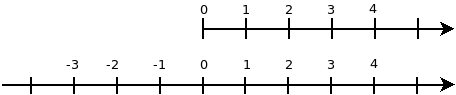
\includegraphics[width=13cm]{allg/alg/img/Zahlenstrahl.png}}
\end{center}

Der Zahlenstrahl hat den Startpunkt 0 (Null)\footnote{... manchmal  den Startpunkt 1 ...}, wohingegen die
Zahlengerade auf beiden Seiten uneingeschränkt weiterläuft.}%% END TALS
\newpage


\subsection{Rationale Zahlen ($\mathbb{Q}$)}
\index{Zahlen!rationale}\index{rationale Zahlen}

\begin{definition}{rationale Zahlen}{}
Zahlen, welche sich als Bruch mit ganzen Zahlen schreiben lassen,
werden als \textbf{rationale Zahlen} bezeichnet.


$$\mathbb{Q} =\left\{ q = \frac{a}{b} \,\,\, \middle| \,\,\, a \in \mathbb{Z}, b \in \mathbb{N}\backslash{}\{0\}\right\}$$
\end{definition}

\subsubsection{Dezimalbrüche}\index{Dezimalbruch}
Jeder Bruch ($\frac{a}{b}$\TRAINER{  $a, b \in \mathbb{Z}, b\ne 0$}) lässt sich als
abbrechender oder periodischer Dezimalbruch schreiben. Beispiel:

Abbrechend:
$$\frac{175}{8} = \LoesungsRaumLang{21.875}$$
Periodisch:
$$\frac{5}{70} = \LoesungsRaumLang{0.0\overline{714285}}$$

Dasselbe gilt umgekehrt. Für abbrechende Dezimalbrüche ist dies
trivial:
$$47.386 = \LoesungsRaumLang{\frac{47\,386}{1\,000}}$$

Für periodische, nicht abbrechende Dezimalbrüche sieht die Sache etwas komplizierter aus,
gilt jedoch auch:

$$0.\overline{13} = 0.131313... = \LoesungsRaumLang{13\cdot{}\frac1{99}=\frac{13}{99} = 13 : 99}$$

\TNTeop{Bem.: $\frac{1}{9} = 0.111\overline{1}$, $\frac{1}{99} = 0.0101\overline{01}$, $\frac{1}{999} = 0.001001\overline{001}$, ...}

%%%%%%%%%%%%%%%%%%%%%%%%%%%%%%%%%%%%%%%%%%%%

  \subsection*{Aufgaben}
  Zeigen Sie, dass die folgenden Dezimalzahlen rational sind. Schreiben Sie dazu diese Zahlen als gewöhnliche, gekürzte Brüche:

  \renewcommand{\arraystretch}{1.5}
  \begin{tabular}{|c|c|c|}
  $0.8=\LoesungsRaum{\frac45}$                  & $-2.03=\LoesungsRaum{-\frac{203}{100}}$         & $2.125=\LoesungsRaum{\frac{17}{8}}$                             \\
  $3.\overline{3}=\LoesungsRaum{\frac{10}{3} }$ & $4.\overline{16}=\LoesungsRaum{\frac{412}{99}}$ & $1.\overline{538461} =\LoesungsRaum{\frac{170\,940}{111\,111}}$ 
  \end{tabular} 
  \renewcommand{\arraystretch}{1}


\TNTeop{}

%%  \GESOAadBMTA{22}{Optional: 6., 7.}
%%  \TALSAadBMTA{8}{Optional: 1., 2.}

%%  \noTRAINER{\mmPapier{6}}%% END noTRAINER

%%%%%%%%%%%%%%%%%%%%%%%%%%%%%%%%%%%%%%%%%%%


\subsection{Runden}\index{runden}
In der Regel sind wir bei Dezimalbrüchen nicht an allen auftretenden
Stellen interessiert, sondern begnügen uns mit einer Näherung.

\subsubsection{Dezimalen (Nachkommastellen)}\index{Dezimale}\index{Nachkommastelle}
Als Dezimalen, Dezimalstellen oder Nachkommastellen werden die Stellen
\textbf{nach} dem Komma bezeichnet.

\begin{rezept}{Runden}{}
  Beim \textbf{Runden} auf die $n$-te Stelle, wird die $n+1$-te Stelle
  betrachtet. Ist diese >=5, so wird \textbf{aufgerundet}, ansonsten \textbf{abgerundet}.
\end{rezept}

Runden auf die vierte \textbf{Dezimale} (= vierte \textbf{Nachkommastelle}):
$$ 36.4699432 \approx  \LoesungsRaum{36.4699}$$
$$ 36.4699618 \approx  \LoesungsRaum{36.4700}$$
\textbf{Vorsicht} bei Zahlen nahe an Null. So wird die Zahl
$$0.002468$$ beim Runden auf vier Dezimalen wie folgt gerundet:
$$0.0025$$

Runden Sie auf {\color{ForestGreen}vier} Dezimalen:

\begin{tabular}{rcl}
  $55.55555$      &$\approx$& \LoesungsRaum{$55.{\color{ForestGreen}\mathbf{5556}}$}\\
  $8.55695$       &$\approx$& \LoesungsRaum{$8.{\color{ForestGreen}\mathbf{5570}}$}\\
  $3.3339499$     &$\approx$& \LoesungsRaum{$3.{\color{ForestGreen}\mathbf{3339}}$}\\
  $1000.0001$     &$\approx$& \LoesungsRaum{$1000.{\color{ForestGreen}\mathbf{0001}}$}\\
  $10\,000.00001$ &$\approx$& \LoesungsRaum{$10\,000.{\color{ForestGreen}\mathbf{0000}}$}\\
  $-6.99999$      &$\approx$& \LoesungsRaum{$-7.{\color{ForestGreen}\mathbf{0000}}$}\\
  $0.000040447$   &$\approx$& \LoesungsRaum{$0.{\color{ForestGreen}\mathbf{0000}}$}\\
\end{tabular}

\TRAINER{Das letzte Beispiel zeigt, dass so oft wichtige Information
  verloren geht. Daher wird sinnvollerweise meist auf signifikante Stellen, und nicht
  auf Dezimalen gerundet.}
\newpage

\subsubsection{Signifikante Stellen\GESO{ (optional)}}\index{signifikante Stellen}
\begin{rezept}{Auf signifikante Ziffern runden}{}
  
  Beim Runden auf \textbf{vier signifikante Ziffern} wird
  \begin{itemize}
  \item  von links nach rechts die erste von Null verschiedene Ziffer gesucht. Dies ist die
    erste signifikante Ziffer.
  \item
    Danach werden die nächsten drei Ziffern
  genommen, egal ob sie Null sind oder nicht. 
\item   Mit diesen drei Ziffern bilden die Ziffern zusammen die vier
  signifikanten Ziffern.
\item  Die 5. Ziffer wird nur noch zum Auf- oder Abrunden verwendet.
  \end{itemize}
\end{rezept}

Geben Sie {\color{ForestGreen}\textbf{vier}} \textbf{signifikante} Ziffern an und runden Sie wenn nötig:

$$0.000040447  \approx \LoesungsRaum{0.0000{\color{ForestGreen}\mathbf{4045}}}$$
$$36.4699432 \approx \LoesungsRaum{{\color{ForestGreen}\mathbf{36.47}}}$$
$$36.9952831 \approx \LoesungsRaum{{\color{ForestGreen}\mathbf{37.00}}}$$
$$30009.78   \approx \LoesungsRaum{{\color{ForestGreen}\mathbf{3001}}0}$$
$$0.0439899  \approx \LoesungsRaum{0.0{\color{ForestGreen}\mathbf{4399}}}$$
$$1\,000\,000 \approx \LoesungsRaum{{\color{ForestGreen}\mathbf{1\,000}}\,000}$$
$$0.00001    \approx \LoesungsRaum{0.0000{\color{ForestGreen}\mathbf{1000}}}$$


\subsection*{Aufgaben}

\aufgabenFarbe{Runden Sie die Zahl 3.21459 auf zwei Dezimalen: \LoesungsRaumLang{3.21}. Runden Sie die selbe Zahl 3.21459 auf drei Dezimalen: \LoesungsRaumLang{3.215} und runden Sie nun das gerundete Resultat auf zwei Dezimalen: \LoesungsRaumLang{3.22}. Was ist davon zu halten?}%% END Aufgabenfarbe

\TNTeop{Rechnen Sie nie mit bereits gerundeten Zwischenresultaten. Der Fehler kann sich dadurch vergrößern!}%% END TNT

%%%%%%%%%%%%%%%%%%%%%%%%%%%%%%%%
  
\subsubsection{Wissenschaftliche Notation}\index{Notation!wissenschaftliche}\label{wissenschaftlicheNotation}
Bei Zahlen größer als 10 können wir einer Zahl manchmal nicht ansehen, wie viel Stellen denn nun signifikant sind.

$$ 679\,946 \textrm{\ Einwohner} \approx  \LoesungsRaumLang{680\,000} \textrm{\ Einwohner}$$
$$ 680\,023 \textrm{\ Einwohner} \approx  \LoesungsRaumLang{680\,000} \textrm{\ Einwohner}$$

Daher bietet sich die wissenschaftliche Notation an.\footnote{Die
\textbf{wissenschaftliche Notation} wird vorwiegend für sehr große
aber auch für Zahlen sehr nahe an Null verwendet.}
Bei der wissenschaftlichen Notation wird die erste signifikante Ziffer
vor das Komma geschrieben. Nach dem Komma stehen \textbf{alle} weiteren signifikanten Stellen.
Zuletzt wird die Zahl mit Zehnerpotenzen
($10^{n}: n \in \mathbb{Z}$) «an die richtige Stelle» gerückt:

$$64\,038.6  = \LoesungsRaumLang{6.40386 \cdot 10^{ 4}} \approx \LoesungsRaumLang{6.40 \cdot 10^{ 4}}$$
$$0.00463640 = \LoesungsRaumLang{4.63640 \cdot 10^{-3}} \approx \LoesungsRaumLang{4.64 \cdot 10^{-3}}$$

Dabei bezeichnen negative Exponenten die Zehntel, Hundertstel, etc.
Erst in der wissenschaftlichen Notation können wir die signifikanten Stellen auch bei gerundeten Zahlen größer als 10 effektiv ablesen.

%%\TALS{S. \cite{frommenwiler17alg} S. 40 Kap. 1.5.5}
\newpage

\paragraph{Taschenrechner} Auf Taschenrechnern oder in
Programmiersprachen wird die Exponentialschreibweise i.\,d.\,R. mit dem
Buchstaben «e» angegeben. Also «e$\color{red}n$» anstelle von «$\cdot10^{\color{red}n}$». Beispiele:

$5\,000 = 5\, \cdot 10^{\color{red}3} = 5\mathrm{e}\color{red}3$

$0.063 = 6.3\, \cdot 10^{-2} = 6.3\mathrm{e-}2$

Berechnen und interpretieren Sie mit dem Taschenrechner:

$$5.7^{15} = \LoesungsRaumLang{2.178e11} = \LoesungsRaumLang{2.178 \cdot{} 10^{11}}$$
$$0.44^{28} =\LoesungsRaumLang{1.039e-10} = \LoesungsRaumLang{1.039\cdot{} 10^{-10}}$$
\begin{rezept}{EE}{}
    Um 5.77 Millionen auf Ihrem Taschenrechner \textbf{einzugeben} tippen Sie:

\begin{center}  \TRAINER{5.77 \GESO{\tiprobutton{EE}}\TALS{\nspirebutton{EE}} 6}\noTRAINER{\vspace{5mm}} \end{center}

\end{rezept}
\GESO{\begin{rezept}{SCI}{}
   Der Taschenrechner kann auch direkt die \textit{Wissenschaftliche Notation}
   anzeigen, wenn er so eingestellt ist:

   Beispiel 0.087 in \textit{Wissenschaftlicher Notation}:

   0.087 \tiprobutton{mode}\texttt{SCI}\tiprobutton{enter}\tiprobutton{2nd}\tiprobutton{mode_quit}\tiprobutton{enter}

   \texttt{8.7E-2} (Dies bedeutet $8.7 \cdot{} 10^{-2}$.)
\end{rezept}
}%% END GESO

Stellen Sie in Wissenschaftlicher Notation dar:

0.00479 $= \LoesungsRaum{4.79 \cdot{}10^{-3}}$

0.08 Milliarden $= \LoesungsRaum{8\cdot{}10^7}$

\newpage

\subsection{Irrationale und reelle Zahlen ($\mathbb{R}$)}\index{Zahlen!reelle}

\youtubeLink{https://www.youtube.com/watch?v=9JgcETAN65c}{Simple-Club:
  Irrationale Zahlen}

\youtubeLink{https://www.youtube.com/watch?v=tPfnEByx9r0}{Dorfuchs: Wurzel zwei ist irrational.}

  Zahlen auf der Zahlengerade, welche nicht als Bruch $\frac{a}{b}$ mit $a\in\mathbb{Z}$, $b \in \mathbb{N}$ dargestellt werden können, werden als \textbf{irrational}\index{irrational} bezeichnet.

Wichtigste Vertreter:

\TNT{5.2}{\bbwCenterGraphic{12cm}{allg/alg/img/IrrationaleZahlen.png}}

\begin{definition}{Reelle Zahl}{}
Die Vereinigungsmenge der rationalen ($\mathbb{Q}$) und der irrationalen Zahlen
nennen wir die \textbf{reellen} Zahlen und bezeichnen die Menge mit $\mathbb{R}$.
\end{definition}


Dass $\pi$ oder $\sqrt{2}$ irrational sind, ist nicht trivial. Daher
noch zwei Vertreter irrationaler Zahlen, bei denen sofort klar ist,
dass es sich nicht um periodische Dezimalbrüche handelt:
\TNTeop{\begin{itemize}
\item $0.10 100 100010000100000100000010000000...$
\item $0.12345678910111213141516 ... 9899100101102103104 ... $
\end{itemize}%%
}%% END TNT

%%%%%%%%%%%%%%%%%%%%%%%%%%%%%%%%%%%%%%%%%%%%

\begin{gesetz}{Zahlmengen Beziehungen}{}
$$\LoesungsRaum{\mathbb{N}} \subset \LoesungsRaum{\mathbb{Z}} \subset
  \LoesungsRaum{\mathbb{Q}} \subset \LoesungsRaum{\mathbb{R}} $$%
\end{gesetz}


\begin{bemerkung}{Mächtigkeit}{}
  Dabei ist $\mathbb{R}$ die mächtigste der vier Mengen. 
\end{bemerkung}

\TNTeop{(Trainer: Beginne beim skizzieren mit $\mathbb{R}$)\\
\bbwCenterGraphic{8cm}{allg/alg/img/nzqr.png}
}%% END TNTeop

%%%%%%%%%%%%%%%%%%%%%%%%%%%%%%%%%%%%%%

\subsection*{Aufgaben zum Kapitel Zahlmengen}

\aufgabenFarbe{Geben Sie jeweils an, zu welchen der Zahlmengen $\mathbb{N}\backslash{}\{0\}$, $\mathbb{Z}$, $\mathbb{Q}$ bzw. $\mathbb{R}$ die folgenden Zahlen gehören:%%
}%% END Aufgabenfarbe

\begin{itemize}
\item $5-8 \LoesungsRaum{\mathbb{Z,Q,R}}$
\item $-3.\overline{17} \LoesungsRaum{\mathbb{Q,R}}$
\item $\sqrt{2.00} - \sqrt{\frac{50}{25}} \LoesungsRaum{\mathbb{Z,Q,R}}$
\item $\frac{3}{\pi} \LoesungsRaum{\mathbb{R}}$
\item $\sqrt{2^5}\LoesungsRaum{\mathbb{R}}$
\item $4.\overline{9} \LoesungsRaum{\mathbb{N,Z,Q,R}}$
\item $3.\overline{18}+\frac{20}{11} \LoesungsRaum{\mathbb{N,Z,Q,R}}$
\item $0.313113111311113111113... \LoesungsRaum{\mathbb{R}}$
\item $\sqrt{-6} \LoesungsRaum{\not\in\mathbb{R}}$
\end{itemize} 

%%\GESOAadBMTA{22ff}{5.}
%%\TALSAadBMTA{9}{4.}

\TNTeop{}

%\newpage
%\subsection{Ordnungsrelationen}\index{Ordnungsrelationen}

\begin{tabular}{c|l}
  $a=b$                        & Gleichheit\noTRAINER{\hspace{20mm}}\\
  $\pi\ne 3$                   & \TNDF{Ungleichheit}\\
  $\pi\approx \frac{355}{113}$ & \TNDF{ungefähr gleich}\\
  $a<b$                        & \TNDF{$a$ ist kleiner als $b$}\\
  $3>1$                        & \TNDF{Analog:  ... ist größer als ...}\\
  $1 \ll 6.022 \cdot{} 10^{23}$ &\TNDF{... sehr viel kleiner als...}\\
  $10^{100} \gg 1000$           & \TNDF{... sehr viel größer als...}\\
  $a\leq b$                    & \TNDF{$a$ kleiner als oder gleich $b$ }\\
  $a\geq 4$                    & \TNDF{Analog: $a$ ist gleich 4 oder größer als 4}  \\
  \hline
\end{tabular}


\subsubsection{Intervall-Notation}

\renewcommand{\arraystretch}3
\begin{tabular}{c|c|c}

  Relation & Zahlenstrahl & Intervallschreibweise \\
  \hline
  $a \geq 4$  &
  \TRAINER{\raisebox{-5mm}{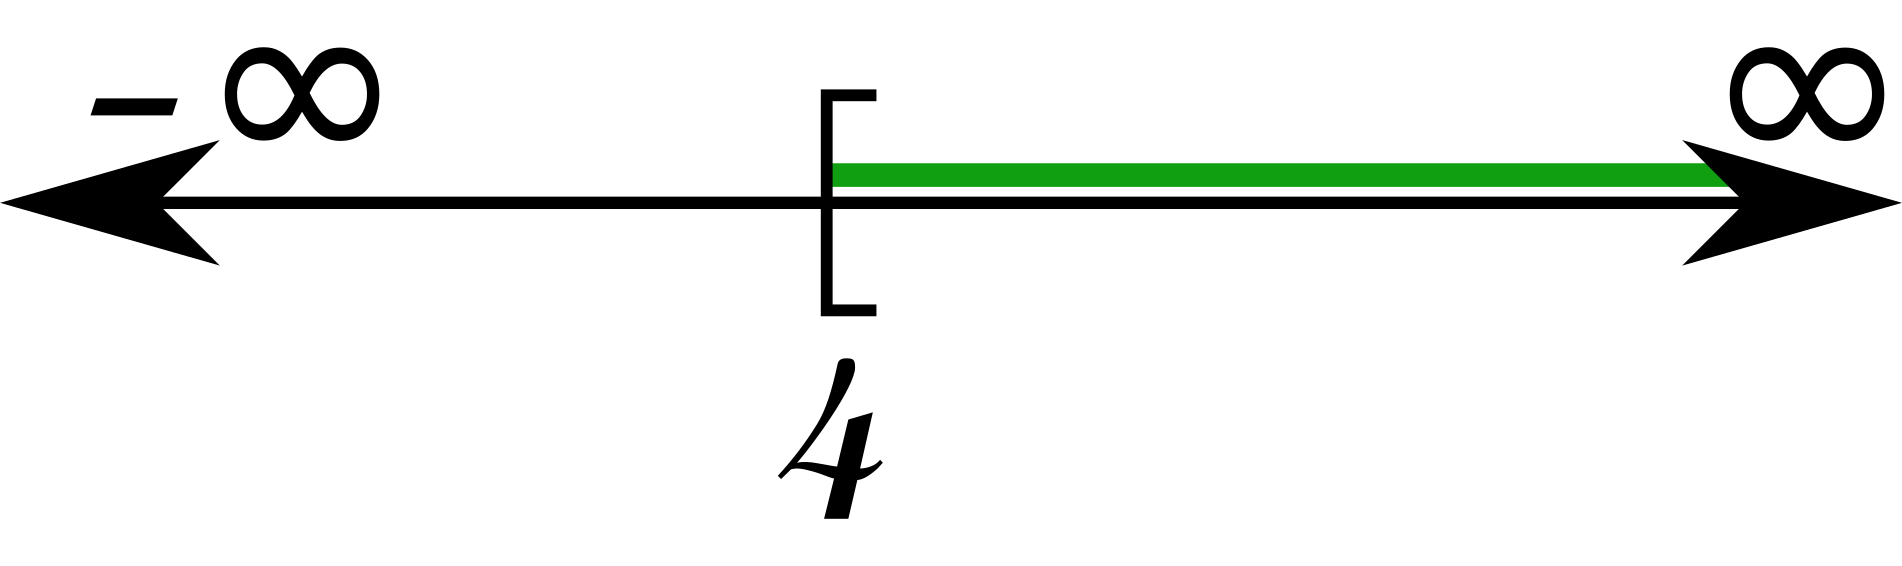
\includegraphics[width=40mm]{allg/alg/img/intervallGE4.png}}}
  \noTRAINER{\hspace{6cm}} & $[4;  \infty [$\\
      \hline
      
  $x\leq 5$ und $x > -2$  &
      \TRAINER{\raisebox{-5mm}{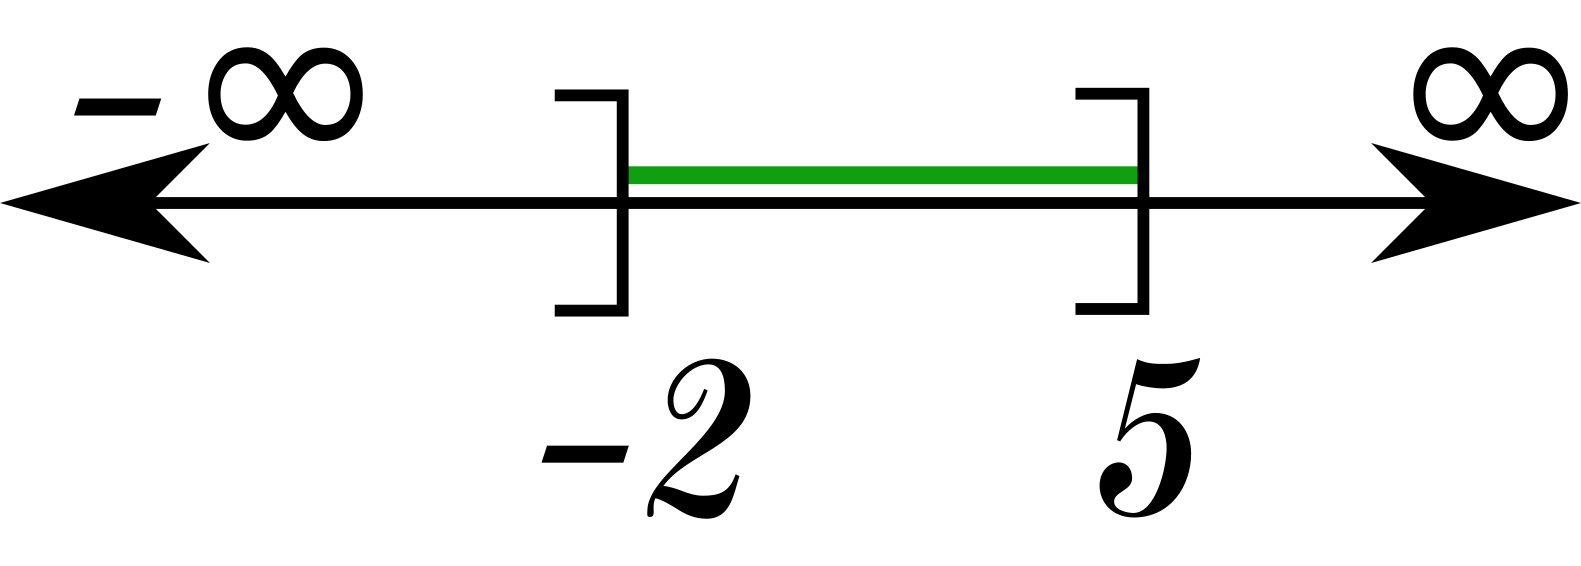
\includegraphics[width=40mm]{allg/alg/img/intervallM2T5.png}}}
      & \TNDF{$]-2; 5]$}\\
  
  \hline
  $-42 > z$  &
  \TRAINER{\raisebox{-5mm}{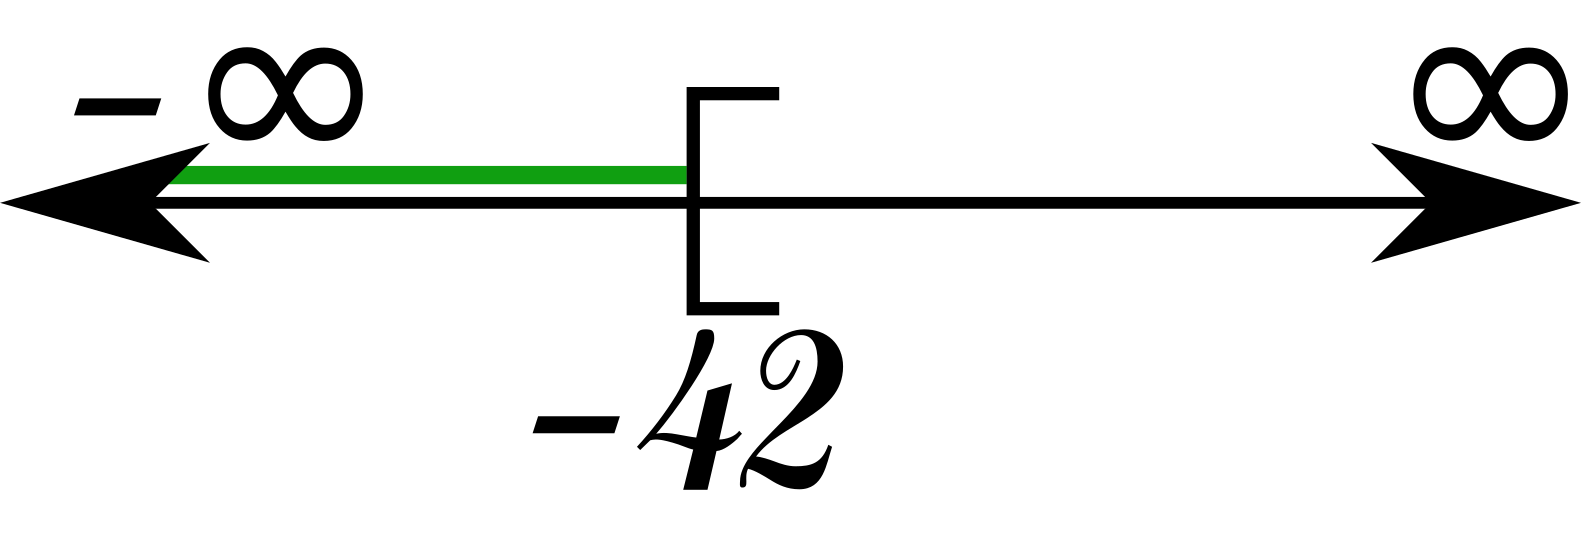
\includegraphics[width=40mm]{allg/alg/img/intervallLE-42.png}}} & \TNDF{$] -\infty ; -42[ $}\\
\hline  
\end{tabular}
\renewcommand{\arraystretch}1
\newpage



\subsection*{Aufgaben zu Ordnungsrelationen}

\aufgabenFarbe{Setzen Sie das richtige Zeichen ($<$, $>$, $=$) zwischen die folgenden Zahlen:}

$\pi \LoesungsRaum{<} \sqrt{10}$ ($\pi$ ist die Kreiszahl)

$-\sqrt{5} \LoesungsRaum{<} \sqrt{2}-\sqrt{13}$

$\frac{10}3 \LoesungsRaum{>} 0.3333333333$

$\e \LoesungsRaum{>} \frac{163}{60}$ ($\e$ ist die Eulersche Zahl)

$8.\overline{9} \LoesungsRaum{=} 18.33 - \frac{933}{100}$

$-\sqrt{6} \LoesungsRaum{\ne} \sqrt{-6}$ \TRAINER{(Fangfrage, denn $\sqrt{-6}$ liegt außerhalb $\mathbb{R}.$)}

\aufgabenFarbe{Ordnen Sie die folgenden Werte der Zahlen bzw. Terme der Reihe nach (auch hier bezeichnet $\e$ die Eulersche Zahl):}

$\pi$, $\frac{10}3$, $\sqrt{10}, \sqrt{3^3}-2, (-2.2)\cdot(-1.5), \e+\frac{41}{50}$

\mmPapier{1.6}

\aufgabenFarbe{Welche der folgenden Aussagen sind wahr (auch hier ist $\e$ die Eulersche Zahl)?}

$\pi > \e$ \TRAINER{Wahr}

$\pi = 3.14$ \TRAINER{Falsch, zwar nur 1/2 Promille daneben, aber
  nicht gleich}

$\pi = 3.14159265$ \TRAINER{Falsch, auch wenn schon besser}

$\pi \approx 3.14259265$ \TRAINER{Falsch, falsche Genauigkeit wird vorgegaukelt}

$0.1\overline{6} < \frac16$ \TRAINER{Falsch, die sind gleich}

$\e \approx 2.7183$ \TRAINER{Wahr, wenn auch nur gerundet}

$-\sqrt{3} < 0 - \sqrt{2}$ \TRAINER{Wahr}

$\sqrt{\frac{8^8}{\e\cdot{}\pi}} > 1.9646 \cdot{} 10^6$ \TRAINER{Wahr}



\TNTeop{}

%%\GESOAadBMTA{22f}{10. b) 11. a) b) c) d)}
%%\TALSAadBMTA{13}{13.}
%%\TRAINER{Spätestens hier auf die Musterlösungswege im OLAT hinweisen.}

%%%
%% 2019 07 04 Ph. G. Freimann
%%

\subsection{Betrag}\index{Betrag}\index{Absolutbetrag}
%%\sectuntertitel{Absolut? Abstand?}
\sectuntertitel{Wo ist negativ positiv? Beim Alkohol-Test!}
\TRAINER{Einstiegsvideos: Daniel Jung und Mathe-Mann}


%%%%%%%%%%%%%%%%%%%%%%%%%%%%%%%%%%%%%%%%%%%%%%%%%%%%%%%%%%%%%%%%%%%%%%%%%%%%%%%%%
\subsection*{Lernziele}

\begin{itemize}
  \item Symbol
  \item Bedeutung als Abstand
  \TALS{\item Gleichungen mit Betrag lösen}
\end{itemize}

%
%\GESOTadBMTA{15}{1.2}%
%\TALSTadBMTA{15}{1.2}%
%
%\BLENDED{\matheNinjaLink{Betrag}{https://olat.bbw.ch/auth/RepositoryEntry/572162163/CourseNode/105951761084932}}

%\newpage
\begin{definition}{Betrag}{definition_betrag}\index{Betrag}\index{Absolutbetrag}
  Unter dem \textbf{Betrag} oder \textbf{Absolutbetrag} einer Zahl versteht man deren (positiven)
  \textbf{Abstand}\index{Abstand} zum Nullpunkt. Das Symbol zum Betrag sind zwei
  senkrechte Striche:\index{$\mid\cdot \mid$ s. Betrag(-striche)}\\
  $|a| := a$, wenn $a$ positiv\\
  bzw.\\
  $|a| := -a$ falls $a$ negativ.
\end{definition}

\begin{bemerkung}{}{}
Mit $|a - b|$ wird der Abstand der Zahlen $a$ und $b$ berechnet. Ist
nämlich $b > a$, so ist die Differenz negativ und wird mit dem
$| \cdot{} |$-Symbol ins Positive gekehrt.
\end{bemerkung}

\begin{bemerkung}{}{}
  Einfach zum Merken: Dem Abstand zwischen zwei Punkten ist egal, in
  welche Richtung er gemessen wird. So liegt Zürich genauso weit von
  Bern entfernt, wie Bern von Zürich entfernt ist. Somit gilt $|a - b| = |b - a|$.
\end{bemerkung}

\GESO{%% TR GESO
  \begin{bemerkung}{}{}
  Auf dem Taschenrechner kann der Absolutbetrag mit \tiprobutton{math}
  «NUM» «abs(...» eingegeben werden.\\
  Tippen Sie:

  \tiprobutton{math} (Pfeil nach rechts) \tiprobutton{enter} 10 - 22 \tiprobutton{enter}

  Sie erhalten $|10-22| = 12$
  \end{bemerkung}
  }%% END GESO
\newpage


\subsubsection{Beispiele}


\TALS{
Für welche Zahlen $x \in \mathbb{R}$ gilt

$|4| = x$ \TRAINER{$x=4$}%

$|4| = -x$ \TRAINER{$x=-4$}%

$|-4| = x$ \TRAINER{$x=4$}

$|-4| = -x$ \TRAINER{$x=-4$}


$|x| = 4$ \TRAINER{$\lx=\{4, -4\}$}%

$|x| = -4$ \TRAINER{$\lx=\{\}$}%

$|-x| = 4$ \TRAINER{$\lx=\{4, -4\}$}%

$|-x| = -4$ \TRAINER{$\lx=\{\}$}%
}

\GESO{
$|4| = \LoesungsRaum{4}$%

$|-4| = \LoesungsRaum{4}$%

  aber:
  
$-|4| = \LoesungsRaum{-4}$%

$-|-4| = \LoesungsRaum{-4}$%

$|8-5| = \LoesungsRaum{3}$%

$|5 -8| = \LoesungsRaum{3}$%

  Achtung:

  $|-5-8| = \LoesungsRaum{13}$

  $|5+8| = \LoesungsRaum{13}$

  
${\big|}|6| - |-10|{\big|} = \LoesungsRaum{4}$%

}

Theorieaufgabe:
$$\big\vert 7 - \left\vert -3 \right\vert \big\vert - |-7-3|$$

\TNT{2.4}{%%
  $ = | 7 - (3) | - | (-7 - 3)|$ \\
  $ =| 4 |       - | -10 |$ \\
  $ = 4 - (+10)$ \\
  $= -6$
}%% END TNT

\TALS{%
  2. Beispiel:

  Für welche $x$ gilt folgendes:
  $$|x - 3| = 8$$

\TNT{2.4}{%%
  Erste Lösung: Welche Zahlen haben von 3 den Abstand 8? Lsg.:
  11 und -5. Formal: 1. Fall $x-3 > 0$, dann ist $x-3=8$ und somit
  $x_1=11$; 2. Fall $x-3 <=0$, dann ist $-(x-3)=8$ und somit $x_2=-5$
}% END TNT
}% 2. Beispiel Theorieaufgabe TALS


\subsection*{Aufgaben}
\GESO{\olatLinkArbeitsblatt{Betrag [A1B]}{https://olat.bbw.ch/auth/RepositoryEntry/572162163/CourseNode/105796974541159}{1. a) bis e) und 2. a) bis g)}}%% END olatLinkArbeitsblatt
\TALS{\olatLinkArbeitsblatt{Betrag [A1B]}{https://olat.bbw.ch/auth/RepositoryEntry/572162090/CourseNode/105796974602793}{1. a) bis e) und 2. a) bis g)}}%% END olatLinkArbeitsblatt


%%Weitere Aufgabe im Buch:
%%\TALSAadBMTA{9}{5. - 7., 14., 16.-18.}
%%\GESOAadBMTA{23}{14. a) b) c) f), 15. a), 17. a) e) und 18. a)}

\newpage

\subsubsection{Kontrolle}
Berechnen Sie:
$$\left| |4-8| - 11 \right| = \LoesungsRaumLang{7}$$

Challenge: Lösen Sie die folgenden Gleichungen nach $x$ auf:

$$|x| = 11.4 \Longrightarrow \lx = \LoesungsRaumLang{\{-11.4; 11.4\}}$$
$$|x-3| = 7 \Longrightarrow \lx = \LoesungsRaumLang{\{-4; 10\}}$$

Für welche Zahlen $x\in\mathbb{R}$ gilt:
$$|-x| = -x$$
$$\mathbb{L}_x = \LoesungsRaumLang{\mathbb{R}^-_0}$$

\youtubeLink{https://www.youtube.com/watch?v=yiJTCL9I-aU}{Mathe Mann/Mathe Frau: Betrag}

\newpage

%%%
%% 2019 07 04 Ph. G. Freimann
%%

\section{Terme}\index{Term}
\sectuntertitel{Römische Bäder?}

%%%%%%%%%%%%%%%%%%%%%%%%%%%%%%%%%%%%%%%%%%%%%%%%%%%%%%%%%%%%%%%%%%%%%%%%%%%%%%%%%
\subsection*{Lernziele}

\begin{itemize}
 \item Termanalyse (Summe, Differenz, Produkt, Quotient, Potenz)
 \item Hierarchie der Terme (Vorrangregeln)
 \item Termumformungen
 \item Ausmultiplizieren
\end{itemize}

%%\TALSTadBFWA{10}{1.1.3}
\TadBMTA{17}{1.3}
%%\TALSTadBMTA{17}{1.3}

\newpage

\subsection{Term-Definition}\index{Term}
\begin{definition}{Term}{definition_term}
  Ein \textbf{Term} ist entweder
  \begin{itemize}
  \item ein Atom (eine Zahl (\zB{} $4.86$) oder  eine Variable (\zB{}
  $a$, $x$))
  \item ein Klammerausdruck (\zB{} \fbox{({\color{green}T})}, inkl.  Wurzeln \fbox{$\sqrt{\color{green}T}$})\footnote{Dabei wird der
  horizontale Strich wie eine Klammer aufgefasst.}
%%  \item weitere \TALS{Monome\index{Monom}}\GESO{Summanden (Teile einer Summe)}:
%%    \begin{itemize}
   \item eine \textbf{Potenz}\index{Potenz}\footnote{Als Exponent darf
     ein beliebiger Term eingesetzt werden, wohingegen als Basis
     lediglich Atome, Klammerausdrücke und Wurzelterme verwendet
     werden dürfen, wegen der Verwechslungsgefahr. Bei
     ${\frac{a}{b}}^c$ ist nämlich nicht klar, wohin das $c$ denn gehört.} (\fbox{${\color{green}T_1}^{\color{green}T_2}$} \zB{} $a^3$, $(2a - 4)^{x+2}$)
    \item  ein Bruchterm\footnote{Wie bei der Wurzel, dient der Bruchstrich als Klammerpaar: $\frac{U}{V}=(U):(V)$} (\fbox{$\frac{\color{green}T_1}{\color{green}T_2}$} \zB{} $\frac{2^x}{x^2}$)
    \item ein implizites \textbf{Produkt}\footnote{Ein implizites
      Produkt ist mit Koeffizienten angereicherter Ausdruck
      \textbf{ohne} Multiplikationszeichen.} (\zB{}
      ${\color{red}4a}{\color{green}T}$)\footnote{Tritt eine Zahl auf,
      so ist diese immer ganz links zu schreiben. Zahlen rechts von
      Ausdrücken werden mit einem Multiplikationszeichen ($\cdot$) versehen: $5x$, aber $x\cdot{}5$.}
    \item ein explizites \textbf{Produkt}\index{Produkt} ($\cdot$;  ${\color{green}T_1}\cdot {\color{green}T_2}$ \zB{} $a\cdot(-1)$) bzw. ein expliziter \textbf{Quotient}\index{Quotient} ($:$, $/$, $\div$; $6a\cdot3b$ bzw. ${\color{green}T_1}:{\color{green}T_2}$ \zB{} $36m^2:12m^2$)
%%    \end{itemize}
  \item eine \textbf{Summe}\index{Summe} (bzw. \textbf{Differenz}\index{Differenz}) von \TALS{Monomen}\GESO{Summanden\index{Summand}}
  (Zum Beispiel bilden die folgenden
  vier «Pakete» eine Differenz):\\
  $-4x^2 + \frac{3a+b}{x} + \sqrt{5y^2-6} - 5t:2t$

    \end{itemize}
(In obiger Aufzählung hat der am höchsten stehende Term die größte
«Bindungskraft». Beispiel «Punkt vor Strich».)
\end{definition}

\textbf{Gegenbeispiele}
Keine Terme sind \zB{}: $x \cdot{}-8$, $\sqrt{+^2}$, $4+*($, $\frac{7}{+}$, $\frac{(a+b}{-c-d)}$.

Generell werden die fünf wichtigsten Termarten in die folgenden drei Kategorien eingeteilt:
\begin{itemize}
\item Potenz
\item Produkt und Quotient
\item Summe und Differenz
\end{itemize}


\newpage

\subsection{Vorrangregeln}\index{Vorrangregeln}

Es gilt Punkt vor Strich. Daneben bindet ein Exponent (\zB $5^8$) noch
stärker. Am stärksten binden Klammern oder horizontale Linien
(Bruchstrich, Wurzelzeichen).

\bbwCenterGraphic{8cm}{allg/alg/img/Klapopustri.png}
\begin{center}
  Das \textit{Klapopustri}\index{Klapopustri} meint dazu:

  \textbf{Klammern} vor \textbf{Potenzen} vor \textbf{Punkt} vor
  \textbf{Strich}
  
\end{center}




Beispiel:
$$-10^4 = \LoesungsRaumLang{-(10^4) = -
  (10\cdot{}10\cdot{}10\cdot{}10) = -10\,000}$$
\newpage

\subsubsection{Terme benennen}
Nicht jeder Term, der ein Pluszeichen enthält, ist automatisch eine
Summe.

Teilen Sie die folgenden Terme in die Kategorie «Summe/Differenz»,
«Produkt/Quotient» und «Potenz/Wurzel» ein. Tipp: Setzen Sie vorab
«unnötige» Klammern und Multiplikationspunkte:


\renewcommand{\arraystretch}{2}
\begin{tabular}{c|c|c}
  Term                       & mit Klammern                        & Zuordnung\\\hline
  $3x^{4-a} - y^{b+2}$ & $\left(3\cdot{}\left(x^{(4-a)}\right)\right) - \left(y^{(b+2)}\right)$  &  Differenz \\\hline
  $ax + 2b$ & \TRAINER{$(a\cdot{}x) + (2\cdot{}b)$} & \TRAINER{Summe}\\\hline
  $\frac{5+x}{5x}$ & \TRAINER{$\frac{(5+x)}{(5\cdot{}x)}$} & \TRAINER{Quotient}\\\hline
  $\sqrt{2x^3+5}$ & \TRAINER{$\sqrt{((2\cdot{}(x^3)) + 5)}$} & \TRAINER{Wurzelterm}\\\hline
  $(a+b)^{c+d}$ & \TRAINER{$(a+b)^{(c+d)}$} & \TRAINER{Potenz}\\\hline
  $(5-3y)c^8$ & \TRAINER{$(5-3\cdot{}y)\cdot{}(c^8)$} & \TRAINER{Produkt}\\\hline
  $(\sqrt{x-3}+\sqrt{8-b})^2$ & \TRAINER{$((\sqrt{(x-3)})+(\sqrt{(8-b)}))^2$} & \TRAINER{Potenz}\\\hline
  $2\cdot{}7^{3-y}$ & \TRAINER{$2\cdot{}\left(7^{(3-y)}\right)$} & \TRAINER{Produkt}\\\hline
  $\frac15-2\cdot{}4^{x+1}$ & \TRAINER{$\frac15-\left(2\cdot{}\left(4^{(x+1)}\right)\right)$} & \TRAINER{Differenz}\\\hline
\end{tabular}

\renewcommand{\arraystretch}{2}
\newpage

\TALS{\TRAINER{
Im Compilerbau (Schreiben einer Programmiersprache) werden die
folgenden Vorrangregeln verwendet:

\begin{itemize}
\item Term :== Summand \{'+'|'-' Summand\}*\\
\TRAINER{$4a^3 - 6\cdot az^{(7+b)} : \sin(30)$}

\item Summand :== ExpilziterFaktor \{'$\cdot$'|'/' ExpliziterFaktor\}*\\
\TRAINER{$4a^3$, $6 \cdot az^{(7+b)} : \sin(30)$}

\item ExpliziterFaktor :== Faktor \{Faktor\}*\\
\TRAINER{$4a^3$, $6$, $az^{(7+b)}$, $\sin(30)$}

\item Faktor :== SkalarOderKlammerausdruck \{${\,}^{Term}$\}?\\
\TRAINER{$4$, $a^3$, $6$, $a$, $z^{(7+b)}$, $\sin(30)$}

\item SkalarOderKlammerausdruck :== Zahl |
           Variable |
           $\sqrt[Term]{Term)}$ | 
           '(' Term ')' |
           $\frac{Term}{Term}$|
           \textit{Funktionsname} '(' Term ')'\\
\TRAINER{$4$, $a$, $3$, $6$, $a$, $z$, $(7+b)$, $\sin(30)$}

\item \textit{Funktionsname} := 'sin', 'cos', 'tan', 'log', 'lg', 'ln', ....
\end{itemize}
}%% END TRAINER
\noTRAINER{\newpage\mmPapier{180mm}}
}%% IND TALS


\TALS{\newpage
\textbf{Achtung} Bei zusammengeschriebenen Faktoren (\zB $ab$) bindet
           die Multiplikation stärker als beim expliziten verwenden
           des Multiplikationszeichens (\zB $a\cdot{}b$). Beispiel
           $a\cdot bm = a\cdot (b\cdot m)$.

Gleich ein Beispiel, wo dies eine Rolle spielt:
$$111x : 37x = (111x) : (37x) = 3$$
Aber
$$111\cdot x : 37\cdot x = ((111 \cdot x) : 37) \cdot x = 3x^2$$
}%% END TALS

\subsection*{Aufgaben}
\AadBMTA{23ff}{21. und 22.}
%\TALSAadBFWA{11}{9.}
%%\TALSAadBMTA{23ff}{21. und 22.}

\TRAINER{Hier auf die Lösungen zum Buch im OLAT aufmerksam machen.}

\TNTeop{}

%%%%%%%%%%%%%%%%%%%%%%%%%%%%%%%%%%%%%%%%%%%%%%%%%

\subsection{Terme mit Namen}
Oft gibt man Termen Namen, um sie einfacher identifizieren und
bezeichnen zu können. So könnte \zB die Oberfläche einer
Konservendose mit $A$ (Area) wie folgt bezeichnet werden, wenn $r$ den
Radius bzw. $h$ die Höhe bezeichnen:

$$A(r, h) = r^2\pi + r^2\pi + 2r\pi{}h$$

Dabei ist $A$ der Name des Terms und $r$ bzw. $h$ sind die Parameter.
\vspace{3mm}
\begin{beispiel}{Werte einsetzen}{beispiel_terme_werte_einsetzen}
  Wir betrachten den Term

  $T({\color{red}a}, {\color{blue}x}) = 5{\color{red}a}{\color{blue}x} - {\color{red}a} + 7$.

  Nun gilt, dass für jeden Parameter im Term (hier ${\color{red}a}$
  bzw. ${\color{blue}x}$) jede Zahl eingesetzt
  werden kann.\leserluft{}

  $T({\color{red}2}, {\color{blue}-3}) = \LoesungsRaumLang{5\cdot{}{\color{red}2}\cdot{\color{blue}(-3)} - {\color{red}2} + 7}$

  Es können auch Terme anstelle der Parameter eingesetzt
  werden\footnote{Beachten Sie, dass beim Einsetzen von Termen in der Regel
  Klammern gesetzt werden müssen!}:\leserluft{}

  $T({\color{red}z-4}, {\color{blue}2y}) =
  \LoesungsRaumLang{5 \cdot{} {\color{red}(z-4)} \cdot {\color{blue}(2y)} - {\color{red}(z-4)} + 7}$
\end{beispiel}

\begin{bemerkung}{}{}
Achten Sie beim Ersetzen des Parameters durch das Argument auf die
Klammersetzung. Wenn nicht sicher: Immer Klammern um die Argumente
setzen, welche für die Parameter eingesetzt werden:

$$ a = z-4$$
$$ a  \rightarrow (z-4)$$
\end{bemerkung}

\begin{gesetz}{Einsetzen}{}
  Beim Einsetzen eines Term in eine Variable sind \textbf{immer} Klammern zu setzen!
\end{gesetz}
\newpage

\subsubsection{Übungsbeispiel}
$$T(b, y) = 7y^2 - 4by$$

Wir berechnen


$T(\underbrace{{\color{blue}s}}_b, \underbrace{{\color{green}-t}}_y) = $%%
\noTRAINER{.......................................................}%%
\TRAINER{$7\cdot (\underbrace{{\color{green}-t}}_{y})^2 - 4\cdot (\underbrace{{\color{blue}s}}_b) \cdot (\underbrace{{\color{green}-t}}_y) = 7t^2+4ts$}

und

$T(x, 2b) = $ \noTRAINER{.........................................................}\TRAINER{$7(2b)^2 - 4\cdot (x) \cdot (2b) = 28b^2 - 8bx =
  4b (7b-2x)$}
\newpage
\subsection*{Aufgaben}

\aufgabenFarbe{Berechnen Sie die Werte der folgenden Terme und kontrollieren Sie anschließend Ihre Resultate mit dem Taschenrechner:}

\begin{tabular}{|c|c|}
  $-10^4$ & $\LoesungsRaum{-10\,000}$\\
  $(-10)^5$ & $\LoesungsRaum{-100\,000}$\\
  $(-100)^2$ & $\LoesungsRaum{+10\,000}$\\
  $x^6\textrm{, für } x=-1$ & $x^6= \LoesungsRaum{+1}$\\
  $-x^5\textrm{, für } x=-10$ & $-x^5= \LoesungsRaum{+100\,000}$\\
  $(-x)^3\textrm{, für } x=-2$ & $(-x)^3= \LoesungsRaum{+8}$\\

  $A(r) = r^2\pi$ & $A(4)=$ \LoesungsRaum{$16\pi\approx{}50.27$}\\
  $T(x) = -x^2\cdot{}x^1$ & $T(3)=$ \LoesungsRaum{$-27$}\\
  $f(x) = -x^2\cdot{}x^3$ & $f(-2)=$ \LoesungsRaum{$+16$}\\
  $D(a;b;c) = b^2-4ac$ & $D(1; -2; -3)=$ \LoesungsRaum{16}\\
\end{tabular}


\newpage
\aufgabenFarbe{Füllen Sie die folgende Tablele aus:}
\begin{tabular}{cccrcc}
  $x$     & 5                       & 3                    &  -1                 & 0\\\hline
  $a$     & 2                       & $\frac12$            &   0                 & -3\\\hline
  $b$     & 0                       & 2                    &  -1                 & 1\\\hline\hline
  $x^2$   & 25                      & \LoesungsRaum{9 }    &  \LoesungsRaum{1}   & \LoesungsRaum{0}\\\hline
  $x^3$   & \LoesungsRaum{125}      & \LoesungsRaum{27}    &  \LoesungsRaum{-1}  & \LoesungsRaum{0}\\\hline
  $-x^2$  & \LoesungsRaum{-25}       & \LoesungsRaum{-9 }   &  \LoesungsRaum{-1}  & \LoesungsRaum{0}\\\hline
  $a-b^2$ & \LoesungsRaum{2}        & \LoesungsRaum{-3.5}  &  \LoesungsRaum{-1}  & \LoesungsRaum{-4}\\\hline
  $10x^2$ & \LoesungsRaum{250}      & \LoesungsRaum{90}    &  \LoesungsRaum{10}  & \LoesungsRaum{0}\\\hline
  $\left(-\frac{b}{-a}\right)$
          & \LoesungsRaum{0}       & \LoesungsRaum{4}      &  \LoesungsRaum{geht nicht}  & \LoesungsRaum{$-\frac13$}\\\hline
  
  
\end{tabular}

Weitere Trainingsaufgaben im Buch. Beispiel:
\AadBMTA{24ff}{26. a) b) c), 27. a) 28. und 29.\GESO{*}}
%%\TALSAadBMTA{24ff}{26. a) b) c), 27. a) 28. und 29.}
\newpage

%%
%% 2019 07 04 Ph. G. Freimann
%%

\subsection{Polynome}\index{Polynom}
\sectuntertitel{Poly = viel; Nom = Name}

\TALSTadBFWA{12}{1.1.4}
\GESOTadBMTA{18}{1.4}
%%%%%%%%%%%%%%%%%%%%%%%%%%%%%%%%%%%%%%%%%%%%%%%%%%%%%%%%%%%%%%%%%%%%%%%%%%%%%%%%%
\subsubsection*{Lernziele}

\begin{itemize}
\item Grad, Grundform und Koeffizienten
\end{itemize}


Eine spezielle Form von Termen sind die
\textbf{Polynome}.\footnote{Siehe dazu auch im Anhang das
  Summenzeichen auf Seite \pageref{Summenzeichen}.}


\begin{beispiel}{Polynom}{}
  
  Binom: $T(x) = \LoesungsRaumLang{5x^4 + 3x}$
  \leserluft{}
  
  Trinom: $T(z) = \LoesungsRaumLang{7bz^6 + \sqrt{2}z^3 + 44}$
  \end{beispiel}


\begin{definition}{Polynom}{definition_polynom}
  Unter einem \textbf{Polynom} verstehen wir einen Term in einer Variable
  $T(x)$ in der Gestalt:

  \begin{tabular}{rrlllll}\index{$\sum{}$ Summe} 
   $T({\color{red}x}) = \sum\limits_{{\color{blue}i}=0}^{n}{{\color{green}a}_{\color{blue}i}{\color{red}x}^{\color{blue}i}}$ &=& ${\color{green}a}_{\color{blue}0}$ &+ ${\color{green}a}_{\color{blue}1}{\color{red}x}$ &+ ${\color{green}a}_{\color{blue}2}{\color{red}x}^{\color{blue}2}$ &+ $...$ &+ ${\color{green}a}_{\color{blue}n}{\color{red}x}^{\color{blue}n}$\\
    &(=& ${\color{green}a}_{\color{blue}0}{\color{red}x}^{\color{blue}0}$ &+ ${\color{green}a}_{\color{blue}1}{\color{red}x}^{\color{blue}1}$ &+ ${\color{green}a}_{\color{blue}2}{\color{red}x}^{\color{blue}2}$ &+ $...$ &+ ${\color{green}a}_{\color{blue}n}{\color{red}x}^{\color{blue}n}$)
\end{tabular}

    \end{definition}
Dabei bezeichnet n ($\in \mathbb{N}$) den \textbf{Grad} des Polynoms,
während die $a_i$ Koeffizienten in $\mathbb{R}$ sind.

\begin{bemerkung}{}{}Bei Polynomen kommt die Variable weder im Nenner, noch im
  Exponenten, noch unter einer Wurzel vor.\end{bemerkung}

\subsection{Nomenklatur}
Polynome ersten Grades (\zB $ 3x-1$) nennen wir \textbf{lineare}
Polynome\index{Polynom!lineares}.

\GESO{Weitere Definitionen zu \textit{quadratischen} und
  \textit{kubischen} Polynomen finden wir im Buch \cite{marthaler21alg}
  auf Seite 19.}

\textbf{Achtung} Kein Polynom ist $x^2 - \sqrt{x}$, denn $x$ kommt in
der Wurzel vor. Ebensowenig ist $x - \frac{5}{x^2}$ ein Polynom, denn
es lässt sich nicht in die Grundform verwandeln.
\newpage


\subsection{Beispiele}

\renewcommand{\arraystretch}{2}
\begin{tabular}{|r|c|l|}\hline
\multirow{2}{*}{$3yx^2 + 3x$} & Binom  in $x$ & $(3y)\cdot{}x^2 + 3\cdot{}x^1$\\\cline{2-3}
                              & Binom  in $y$ & $(3x^2)\cdot{}y^1 + (3x)\cdot{}y^0$\\\hline
$3m$                    & \LoesungsRaum{Monom in $m$} & \LoesungsRaumLang{$3\cdot{} m^1$}\phantom{xxxxxxxxxxxxxxxx}\\\hline
$4m^2 + 3m$             & \LoesungsRaum{Binom  in $m$} & \LoesungsRaumLang{$4\cdot{}m^2 + 3\cdot{} m^1$}\\\hline
$5t^2 + 2$              & \LoesungsRaum{Binom  in $t$} & \LoesungsRaumLang{$5\cdot{}t^2 + 2\cdot{}t^0$}\\\hline
\multirow{3}{*}{$5a^2 + 4am +2rm + m^3$} & \LoesungsRaum{Trinom in $a$} & \LoesungsRaumLang{$5\cdot{}a^2 + 4m\cdot{}a^1 + (2rm+m^3)\cdot{}a^0$}\\\cline{2-3}
                        & \LoesungsRaum{Trinom in $m$} & \LoesungsRaumLang{$1\cdot{}m^3 + (4a+2r)\cdot{}m^1 + 5a^2\cdot{}m^0$}\\\cline{2-3}
                        & \LoesungsRaum{Binom  in $r$} & \LoesungsRaumLang{$2m\cdot{}r^1 + (5a^2+4am+m^3)\cdot{}r^0$}\\\hline
\end{tabular} 
\renewcommand{\arraystretch}{1}

\subsection*{Aufgaben}
\TALSAadBMTA{13}{10 und 11}
\GESOAadBMTA{25}{30-33}

%%%
%%
\newpage
\section{Grundoperationen}\index{Grundoperationen}
\renewcommand{\bbwAufgabenBlockID}{A1G}
\sectuntertitel{Im Grunde ganz einfach?}

%%%%%%%%%%%%%%%%%%%%%%%%%%%%%%%%%%%%%%%%%%%%%%%%%%%%%%%%%%%%%%%%%%%%%%%%%%%%%%%%%
\subsection*{Lernziele}
\begin{itemize}
\item Addition\index{Addition}, Subtraktion\index{Subtraktion}
\item Multiplikation\index{Multiplikation}
\item Distributivgesetz\index{Distributivgesetz},
  Assoziativgesetz\index{Assoziativgesetz},
  Kommutativgesetz\index{Kommutativgesetz}
\end{itemize}

%%\TALSTadBFWA{15}{1.2}
\TadBMTA{28}{2}
%%\TALSTadBMTA{28}{2}
\newpage

\subsection{Addition und Subtraktion}\index{Addition}\index{Subtraktion}
\begin{beispiel}{}{}
  $$x^2-((x^3-x^2)-(-(-x+x^2)-(x^2-x^3)))$$
\end{beispiel}

\TNT{10}{\bbwCenterGraphic{14cm}{allg/alg/img/KlammernLoesen.png}}%% END TNT

Regeln:
\begin{itemize}
\item Klammern werden von innen nach außen aufgelöst.
\item Gleichwertige Operationen\footnote{Zum Beispiel alles Minus und Plus oder aber zum Beispiel alles \textit{Punkt}-Operationen (Produkt/Quotient).} werden von links nach rechts \textit{geklammert}:
  $$10-4+5 = (10-4) + 5 \ne 10-(4+5)$$
\item Negative Vorzeichen vor Klammern wechseln die Vorzeichen der
      Summanden innerhalb der Klammer.
\item Es können nur gleiche Variable (bzw. Produkte von Faktoren)
      addiert (bzw. subtrahiert) werden.
\end{itemize}

\newpage

\subsection*{Aufgaben}
%%\GESOAadBMTA{34}{1. a) c) e) g), 2. a) e), 3. b), 5. a) f) und 6. d) h)}
%%\TALSAadBMTA{15}{19.}
\GESO{\olatLinkArbeitsblatt{Grundoperationen [A1G]}{https://olat.bbw.ch/auth/RepositoryEntry/572162163/CourseNode/105796961619595}{1. und 2.}}
\TALS{\olatLinkArbeitsblatt{Grundoperationen [A1G]}{https://olat.bbw.ch/auth/RepositoryEntry/572162090/CourseNode/105796961688601}{1. und 2.}}


\newpage
\subsection{Multiplikation}\index{Multiplikation}
\TadBMTA{29}{2.2}
%%\TALS{Theorie im Buch \cite{frommenwiler17alg} S. 16 Kap. 1.3}

Für die Addition und die Multiplikation gelten die drei folgenden
Gesetze:



\begin{gesetz}{}{}
\begin{itemize}
\item  Assoziativgesetz:
  $a+(b+c) = (a+b) +c$ und $a\cdot(b\cdot{}c) = (a\cdot b)\cdot c$
\item Kommutativgesetz:
  $a+b = b+a$ und $a\cdot b = b \cdot a$
\item Distributivgesetz\footnote{lat. \textit{\textbf{distribuere}} = verteilen}:\\
  $a\cdot (b+c) = a\cdot b + a\cdot c$\\
  $a\cdot (b-c) = a\cdot b - a\cdot c$\\
  $(a+b)\cdot c = ac + bc$\\
  $(a-b)\cdot c = ac - bc$\\
  $(a+b):c = a:c + b:c$\\
  $(a-b):c = a:c - b:c$\\
  
  \end{itemize}
\end{gesetz}

\newpage

\subsubsection{Ausmultiplizieren}\index{ausmultiplizieren}
Beim Ausmultiplizieren wird jeder Summand in der Klammer mit dem
Faktor vor (bzw. nach) der Klammer multipliziert.
\begin{beispiel}{}{}
  $4\cdot (x + 5) =\LoesungsRaumLang{4\cdot x + 4\cdot 5 = 4x + 20}$
\end{beispiel}

\begin{beispiel}{}{}
  \noTRAINER{$$(x + 7)\cdot(8-y) = x\cdot(8-y) + 7\cdot(8-y) =
  8x-xy+56-7y$$}\TRAINER{\bbwCenterGraphic{15cm}{allg/alg/img/DistributivRechts.png}}
oder \TRAINER{\\}
  \noTRAINER{$$(x + 7)\cdot(8-y) = (x+7)\cdot 8 - (x+7)\cdot y = 8x+56-xy-7y$$}\TRAINER{\bbwCenterGraphic{15cm}{allg/alg/img/DistributivLinks.png}}
\end{beispiel}

\subsubsection{Kein Distributivgesetz bei Multiplikation eines Produktes}
Berechnen Sie

$$a\cdot{}(4+b) = \LoesungsRaumLang{4a + ab}$$
 ... und ...
$$ a\cdot{}(4\cdot{}b) = \LoesungsRaumLang{4ab} $$

\newpage

\subsubsection{Achtung}
Auch wenn die folgenden Ausdrücke sehr ähnlich aussehen, so
handelt es sich beim ersten um eine \textbf{Differenz} und bei den anderen um
ein \textbf{Produkt}!

$$10-(x-4) =\LoesungsRaum{14-x}$$

$$-10(x-4) = \LoesungsRaum{-10x + 40}$$

$$-10(x\cdot{}(-4)) = \LoesungsRaum{40x}$$

Diese Unterschied wird auf dem Taschenrechner besonders gut deutlich:

\tiprobutton{7}\tiprobutton{minus}\tiprobutton{3}  \tiprobutton{enter}  $ 7 - 3 = 4$

\vspace{3mm}
\tiprobutton{7}\tiprobutton{neg}\tiprobutton{3} \tiprobutton{enter}  $ 7\cdot{}(-3) = -21$


\subsubsection{Referenzaufgabe}
$$3ab-(x-a(2-b))\cdot{}3$$

\TNT{6}{$$3ab-(x-2a+ab)\cdot{}3$$
$$3ab - (3x -6a +3ab)$$
$$3ab - 3x +6a -3ab$$
$$6a-3x$$}
\newpage

\subsection*{Aufgaben}
%%\olatLinkArbeitsblatt{Grundoperationen [A1G]}{\GESO{https://olat.bbw.ch/auth/RepositoryEntry/572162163/CourseNode/105796961619595}\TALS{https://olat.bbw.ch/auth/RepositoryEntry/572162090/CourseNode/105796961688601}}{3., 4. und 5.}
\GESO{\olatLinkArbeitsblatt{Grundoperationen [A1G]}{https://olat.bbw.ch/auth/RepositoryEntry/572162163/CourseNode/105796961619595}{3., 4. und 5.}}
\TALS{\olatLinkArbeitsblatt{Grundoperationen [A1G]}{https://olat.bbw.ch/auth/RepositoryEntry/572162090/CourseNode/105796961688601}{3., 4. und 5.}}
%%\aufgabenFarbe{Aufgaben zu Grundoperationen im OLAT Aufg. [A1G] 3., 4. und 5.}
\newpage
%%\subsection*{Aufgaben}
%%\TALSAadBMTA{16}{21. a) d)}
%%\GESOAadBMTA{34ff}{8. a) d) f) g) 9. c) 12. a) c) e) 13. c) d) 14. g) 16. b) 17. a) 18. d)}


\subsubsection{Minus mal Minus (optional)}
Wir können uns vorstellen, dass $3 \cdot (-4)$ dasselbe ist wie $(-4) + (-4) + (-4)$. Daher gilt
\begin{itemize}
\item $3 \cdot 4 = 12$
\item $3 \cdot (-4) = (-12)$
\item $(-3) \cdot 4 = (-12)$
\end{itemize}
Warum soll aber $(-3)\cdot(-4)$ gleich $+12$ sein?

Hier einige Erklärungsversuche:


\paragraph{Negativer Krankheits-Befund}
Wer negativ auf einen schlimmen Virus- oder Bakterienbefall getestet wurde, kann
die sich doch in einer positiven Situation sehen.

\paragraph{Vorzeichen:} Sehen wir die Zahl $(-4)$ als Gegenzahl von $4$, so können wir auch die Gegenzahl der Gegenzahl betrachten:
$4 = -(-4) = -(1\cdot(-4)) = (-1)\cdot(-4)$. Somit ist $(-1)\cdot(-4) = +4$.

\paragraph{Rechengesetze einhalten:} Wir versuchen den Rechengesetzen, die wir von den positiven Zahlen her kennen, Allgemeingültigkeit zu verleihen, dann müssen sie auch für die negativen Zahlen gelten.
Somit ist
$$(-4)          \cdot 0 = 0$$
Null anders schreiben:
$$(-4)    \cdot (3-3) = 0$$
Gegenzahl addieren:
$$(-4)\cdot(3 + (-3)) = 0$$
Distributivgesetz:
$$(-4)\cdot3 + (-4)\cdot (-3) = 0$$
Term $(-4)\cdot3$ ausrechnen:
$$-12 + (-4)\cdot (-3)= 0$$
Der Gleichung links und rechts 12 hinzufügen (addieren):
$$(-4)\cdot (-3) = 12$$
\newpage

\paragraph{Schuldscheine abgeben:}
Eine anschauliche, aus dem Leben gegriffene, Analogie ist das «Verschenken von Schuldscheinen». Bezeichnen wir Banknoten als Kreditscheine, so besitzt eine 50er Note einen Wert von $+50$. So hat ein Schuldschein von $50.-$ Franken (oder Euros) den Wert $(-50)$.

\begin{tabular}{r@{}l|rl|r@{}l}
Geldwert & Gewinn/Verlust & Effekt\\
\hline\\
 + 50&.--   (Banknote)     &  3&  (erhalten)  & + 150&.-- (Gewinn)   \\
 - 50&.--   (Schuldschein) &  3&  (erhalten)  & - 150&.-- (Verlust)  \\
 + 50&.--   (Banknote)     & -3&  (abgeben)   & - 150&.-- (Verlust)  \\
 - 50&.--   (Schuldschein) & -3&  (abgeben)   & + 150&.-- (Gewinn)   \\
\end{tabular}
\newpage

%%%
%% 2019 07 04 Ph. G. Freimann
%%
\newpage
\section{Binomische Formeln}\index{Formeln!binomische}\index{Binomische Formeln}

\sectuntertitel{2: Zwei, bi-, di-, zwie-, doppel, binär, duo, dual,
Boole'sch, paar, stereo, sekund-, ...\footnote{Zürich unterscheidet die Zahl
2 je nach Geschlecht: «zwoo Fraue», «zwéé Mane» und «zwäi Chinde»}}

\youtubeLink{https://www.youtube.com/watch?v=nSmlfe-ftTo}{Binomische
Formeln (10:37)}
\youtubeLink{https://www.youtube.com/watch?v=zYVY0nmGnbE}{Binomische
Formeln Daniel Jung (4:07)}
        

%%%%%%%%%%%%%%%%%%%%%%%%%%%%%%%%%%%%%%%%%%%%%%%%%%%%%%%%%%%%%%%%%%%%%%%%%%%%%%%%%
\subsection*{Lernziele}

\begin{itemize}
\item Erste:  $(a+b)^2$ 
\item Zweite: $(a-b)^2$
\item Dritte: $(a+b)(a-b)$
\item $1-x^2 = (1+x)\cdot{}(1-x)$

%%  \item Polynomdivision

\end{itemize}

%% \TALSTadBFWA{16}{1.3.1}
\TadBMTA{29}{2.2.1}
%%\TALSTadBMTA{29}{2.2.1}


\newpage


\subsection{Binomische Formeln}\index{Formeln!binomische}
Es gilt:

\TNT{4}{
  $(a+b)\cdot(c+d) = \overbrace{(a+b)}^{X} \cdot (c+d)
  =X(c+d)
  =Xc + Xd
  =(a+b)c + (a+b)d
  =ac + bc + ad + bd$
  \vspace{2cm}
}%% END TNT

Daraus folgen die drei binomischen Formeln
\begin{gesetz}{Binomische Formeln}{}
$$(a+b)^2 = a^2 + 2ab +b^2$$
\vspace{0.01mm}
$$(a-b)^2 = a^2 - 2ab +b^2$$
\vspace{0.2mm}
$$(a+b)(a-b) = a^2 - b^2$$
\end{gesetz}


Graphischer Beweis der 1. binomischen Formel:

%% Für Millimeterpapier siehe auch hier:
%%     http://www.texample.net/tikz/examples/graph-paper/


\TNT{5.2}{%
\raisebox{-1cm}{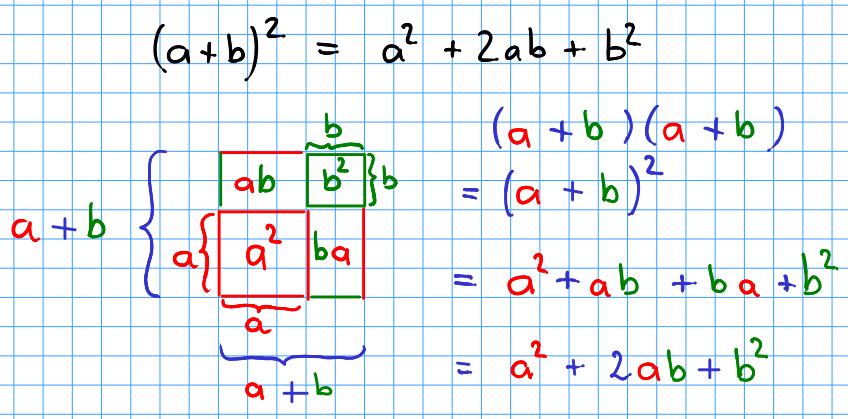
\includegraphics[width=12cm]{allg/alg/img/a_plus_b_zum_quadrat.png}}%
}%% END TNT

\begin{beispiel}{}{}

Typische Anwendungen der binomischen Formeln:

$$(x+5)\cdot(x-5)=\LoesungsRaum{x^2 -25}$$
$$(t+1)\cdot(t-1)=\LoesungsRaum{t^2 - 1}$$
$$(x-2)\cdot(x-2)=\LoesungsRaum{x^2 -4x + 4}$$
\end{beispiel}


\newpage

%Mit diesem Wissen lassen sich einige Summen einfacher ausklammern:
%\vspace{4cm}
%\TRAINER{
%  $$49 - x^2 = (7-x)\cdot(7+x)$$
%  $$a^2 -16a + 64 = (a-8)^2$$
%}

\TALS{
\subsection{Pascalsches Dreieck}\index{Pascalsches
  Dreieck}\index{Dreieck!Pascalsches}

Berechnen Sie $(a+b)^4$:

\TNT{4}{$a^4 + 4a^3b + 6a^2b^2 + 4ab^3 + b^4$}%% END TNT

Zeichnen Sie das Pascalsche Dreieck:
\begin{center}
\begin{tabular}{cccccccccccc}\\
  &   &     &     &     & 1   &     &     &     &     &    & \\
  &   &     &     & 1   &     & 1   &     &     &     &    & \\  
  &   &     & 1   &     & 2   &     & 1   &     &     &    & \\
  &   &  1  &     & 3   &     & 3   &     & 1   &     &    & \\
  & 1 &     & ... &     & ... &     & ... &     & ... &    & \\ 
1 &   & ... &     & ... &     & ... &     & ... &     & ...&  
\end{tabular}
%\noTRAINER{\vspace{3cm}}
\end{center}
\newpage
}


\subsection*{Aufgaben}
%% \TALSAadBMTA{16}{22a) b) e)}
%% \TALSAadBMTA{17}{23a) 24a)}
%% \GESOAadBMTA{36ff}{ 19. b) d) h) 20. a) b) c) d) e) 21. a) 23. a)
%% 24. a) 25. b) e) Optional: 27. c)}
\GESO{\olatLinkArbeitsblatt{Binomische Formeln [A1Bi]}{https://olat.bbw.ch/auth/RepositoryEntry/572162163/CourseNode/105796980058302}{1.) und 2.)}}

\TALS{\olatLinkArbeitsblatt{Binomische Formeln [A1Bi]}{https://olat.bbw.ch/auth/RepositoryEntry/572162090/CourseNode/105796978456639}{1.) und 2.)}}

%%\aufgabenFarbe{Aufgabenblatt im OLAT zu Algebra 1: Binomische
%%Formeln. Aufgaben A1Bi: 1) und 2)}

%%weiter in Algebra II
%%
%% 2019 07 04 Ph. G. Freimann
%%
\newpage
\section{Faktorisieren}\index{Faktorisieren}

%%%%%%%%%%%%%%%%%%%%%%%%%%%%%%%%%%%%%%%%%%%%%%%%%%%%%%%%%%%%%%%%%%%%%%%%%%%%%%%%%
\subsection*{Lernziele}

\begin{itemize}
\item ausklammern
 \begin{itemize}
  \item gemeinsame Faktoren ausklammern
  \item Klammerausdrücke ausklammern
   \begin{itemize}
   \item mehrmaliges Ausklammern (Teilsummen)
  \item -1 ausklammern
  \end{itemize}
\end{itemize}
\item Binomische Formeln
\item Zweiklammeransatz
\TRAINER{\item \textit{(Polynomdivision: kein Lernziel)}}
\item Gemischte Anwendungen
\end{itemize}

%%\TALSTadBFWA{18}{1.3.2}
\TadBMTA{32}{2.2.3}

\newpage


Beim Faktorisieren werden Summen/Differenzen in Faktoren
zerlegt.

\bbwCenterGraphic{11cm}{allg/alg/img/faktorisieren.png}\index{faktorisieren}\index{ausmultiplizieren}

\subsection*{Fernziel und Nutzen des Faktorisierens}
Betrachten wir die beiden folgenden Bruchterme:
 $$\frac{3x(a^2p - pb^2) - 7pa^2 + 7b^2p}{3a^2xy  + 3yb^2x + 6abyx - 7y(a^2 +b^2) - 14ayb }$$
und
$$\frac{p(3x-7)(a+b)(a-b)}{y(3x-7)(a+b)(a+b)}$$

Beide Terme können durch Termumformungen ineinander übergeführt werden. Mit anderen Worten: Die Terme sind identisch. Doch nur dem zweiten können wir auf einen Blick ansehen, dass er durch Kürzen stark vereinfacht werden kann:

$$\frac{p(a-b)}{y(a+b)}$$

%%%%%%%%%%%%%%%%%%%%%%%%%%%%%%%%%%%%%%%%%%%%%%%%%%%%%%%%%%%%%%%%%%%%%%%%%%%%%%%%%%%%%%%%%%%%%%%%%%%%%
\newpage

\subsection{Ausklammern}\index{ausklammern}
Die gängigste Methode des Faktorisierens ist das Ausklammern.

Das \textbf{Ausklammern}\footnote{Ausklammern wird auch «Vorklammern»\index{Vorklammern!Ausklammern} genannt.} ist die einfachste Umkehrung des Ausmultiplizierens.
Dabei werden gemeinsame Faktoren gesucht und vor (bzw. hinter) eine
neu hinzugefügte Klammer geschrieben.

\subsubsection{gemeinsame Faktoren ausklammern}
Suche gemeinsame Faktoren (Variable, Zahlen) in allen Summanden:

\begin{beispiel}{}{}
  $$4a^3 + 2ab -6a^2x$$
  $$=\noTRAINER{\hspace{7em}}\TRAINER{ {\color{green}2a}\cdot{\color{green}(}2a^2+b -3ax{\color{green})}}$$
\end{beispiel}

\begin{beispiel}{Woher kommt die Eins?}{}

$$4a^3 + 2a^2$$
$$=\noTRAINER{\hspace{7em}}\TRAINER{2a^2(2a + 1)}$$
Wenn wir die Faktoren zurück ausmultiplizieren, sehen wir, dass die
Eins (1) nicht fehlen darf. \textbf{Tipp}: Zur Probe immer zurück ausmultiplizieren.
\end{beispiel}




\newcommand{\olatAB}[2]{\subsection*{Aufgaben}
\aufgabenFarbe{OLAT #1. Aufg. #2}
\platzFuerBerechnungenBisEndeSeite{}}

%%\olatAB{Algebra I Faktorisieren Aufgabenblatt A1F}{1}

\GESO{\olatLinkArbeitsblatt{Faktorisieren [A1F]}{https://olat.bbw.ch/auth/RepositoryEntry/572162163/CourseNode/105796980169261}{1.)}}

\TALS{\olatLinkArbeitsblatt{Faktorisieren [A1F]}{https://olat.bbw.ch/auth/RepositoryEntry/572162090/CourseNode/105796978494157}{1.)}}



%%\GESO{\aufgabenFarbe{S. 38: Aufg. 37. 38. a) e) }}
\newpage


\subsubsection{Minus Eins ausklammern I}

\textbf{Vertauschte Differenz}\\

$$8-a = \LoesungsRaumLang{\mathbf{(-1)\cdot{}} (-8 + a) = -(a-8)}$$

Anwendung:
$$\frac{a-3}{3-a} = \LoesungsRaumLang{\frac{(-1)\cdot{}(-a+3)}{3-a}} = \LoesungsRaumLang{\frac{(-1)\cdot{}(3-a)}{3-a}} = \frac{-1}1 = -1$$

Aus jeder Summe (bzw. Differenz)
kann minus Eins $(-1)$ ausgeklammert werden, indem alle Vorzeichen der
Summanden umgedreht werden:

$$ -4 + x - 5\cdot(a-b) +c  =\LoesungsRaumLang{ {\color{ForestGreen} (-1)}\cdot{} ({\color{ForestGreen}+}4 {\color{ForestGreen}-}x {\color{ForestGreen}+}
5\cdot{(a{\color{red}-}b)} {\color{ForestGreen}-}c)}$$

Achtung oben: Das Vorzeichen bei $a-b$ ändert sich nicht, denn dies
ist nicht ein Vorzeichen der globalen Summanden!

%%\subsection{Aufgaben}
%%\GESOAadBMTA{39}{39. h) i)}
%%\GESOAadBMTA{39}{40. a)}

%%\olatAB{Algebra I Faktorisieren Aufgabenblatt A1F}{2}
\GESO{\olatLinkArbeitsblatt{Faktorisieren [A1F]}{https://olat.bbw.ch/auth/RepositoryEntry/572162163/CourseNode/105796980169261}{2.)}}

\TALS{\olatLinkArbeitsblatt{Faktorisieren [A1F]}{https://olat.bbw.ch/auth/RepositoryEntry/572162090/CourseNode/105796978494157}{2.)}}

\newpage


\subsubsection{Identische Klammerausdrücke}\index{Klammerausdruck ausklammern}
Anstelle einfacher Monome können auch ganze Klammerausdrücke
ausgeklammert werden:
$$7x{\color{green}(3+b)} + 5z{\color{green}(b+3)}$$
$$=(7x+5z){\color{green}(3+b)}$$

Tipp: Geben Sie dem Klammerausdruck einen Namen\footnote{Dieser
chinesische Rechentrick löst manches {\color{green}A} bzw. {\color{green}Aha}-Erlebnis aus!}: ${\color{green}A} = {\color{green}(3+b)}$, dann liest sich der
Term wie folgt:
$$7x{\color{green}(3+b)} + 5z{\color{green}(b+3)} = 7x\cdot{\color{green}A}
+ 5z\cdot{\color{green}A} {\stackrel{\textrm{a.}}{=}}
(7x+5z)\cdot{\color{green}A} = (7x+5z){\color{green}(3+b)}$$

\begin{beispiel}{}{}
$$6b(5+x) - x- 5$$
\TNT{5.2}{
$$6b(5+x) -(x+5)$$
$$6b(5+x) -1(x+5)$$
$$6b(x+5) -1(x+5)$$
$$(x+5) (6b-1)$$
}

\end{beispiel}

%\olatAB{Algebra I Faktorisieren Aufgabenblatt A1F}{3}

\GESO{\olatLinkArbeitsblatt{Faktorisieren [A1F]}{https://olat.bbw.ch/auth/RepositoryEntry/572162163/CourseNode/105796980169261}{3.)}}

\TALS{\olatLinkArbeitsblatt{Faktorisieren [A1F]}{https://olat.bbw.ch/auth/RepositoryEntry/572162090/CourseNode/105796978494157}{3.)}}

\newpage



\subsubsection{Minus Eins ausklammern II}\index{Minus Eins ausklammern}
Unterscheiden sich Teilklammern nur durch Vorzeichen, so bietet es
sich an, Minus Eins (-1) auszuklammern, um identische Klammerausdrücke
zu erhalten:
$$7x{\color{green}(b-3)} + 5z{\color{green}(3-b)}$$%%

\TRAINER{%%

$7x{\color{green}(b-3)} - 5z{\color{green}(-3+b)}$
\vspace{10mm}
}%%

\TRAINER{%%

$7x{\color{green}(b-3)} - 5z{\color{green}(b-3)}$
\vspace{10mm}
}%%


\noTRAINER{\mmPapier{3.6}}


%\olatAB{Algebra I Faktorisieren Aufgabenblatt A1F}{4}

\GESO{\olatLinkArbeitsblatt{Faktorisieren [A1F]}{https://olat.bbw.ch/auth/RepositoryEntry/572162163/CourseNode/105796980169261}{4.)}}

\TALS{\olatLinkArbeitsblatt{Faktorisieren [A1F]}{https://olat.bbw.ch/auth/RepositoryEntry/572162090/CourseNode/105796978494157}{4.)}}


%%\TALSAadBMTA{18}{29. b), 30. a) c) d) g), 31. a) c) f), i) und 32. b) f)}
%%\GESOAadBMTA{39}{41. a) e) d) 42. b) c) 43. b) c) 44. b) e) }
\newpage



\subsubsection{Mehrmaliges Ausklammern:}\index{ausklammern!mehrmaliges}
 Um identische Klammerausdrücke zu finden, bietet sich die Methode des mehrmaligen Ausklammerns an.
 Dabei wird die Summe (bzw. Differenz) in gleiche Anzahl \textbf{Teilsummen}\index{Teilsummen} aufgeteilt und Stückweise ausgeklammert.
 Im folgenden Beispiel werden die beiden ersten Summanden und die beiden letzten «Summanden» zunächst unabhängig voneinander betrachtet.

$$3mk+6nk-5m-10n $$
$$= 3k{\color{green}(m+2n)}-5{\color{green}(m+2n)} $$
$$= (3k-5){\color{green}(m+2n)}$$


\begin{beispiel}{}{}
  $$5a-30+ax-6x = ...$$
  Wie gehen wir vor? Beispiel: Aus den ersten beiden Summanden 5 und
  aus den beiden hinteren Summanden $x$ ausklammern:

\TNT{2.4}{$$... = 5\cdot(a-6) + x\cdot(a-6) = ...$$}

  Nun aus beiden Summanden den Term ......... \TRAINER{$(a-6)$}
  ausklammern:

\TNT{2.4}{$$... = (5+x)\cdot(a-6)$$}
\end{beispiel}

%%\olatAB{Algebra I Faktorisieren Aufgabenblatt A1F}{5}
\GESO{\olatLinkArbeitsblatt{Faktorisieren [A1F]}{https://olat.bbw.ch/auth/RepositoryEntry/572162163/CourseNode/105796980169261}{5.)}}

\TALS{\olatLinkArbeitsblatt{Faktorisieren [A1F]}{https://olat.bbw.ch/auth/RepositoryEntry/572162090/CourseNode/105796978494157}{.)}}

\newpage


\subsection{Binomische Formeln}\index{Faktorisieren!mit binomischen Formeln}%%
\index{Binomische Formeln!zum Ausklammern}



Zerlegen wir die folgenden Terme in einzelne Faktoren:
$$ a^2 - 16 = \LoesungsRaum{(a+4)(a-4)} $$

$$x^2 -18x + 81 = \LoesungsRaum{(x-9)(x-9)}$$

$$64y^2 - 49z^6 = \LoesungsRaum{(8y+7z^3)(8y-7z^3)}$$

$$c^4 - 1 = \LoesungsRaum{\mathbf{(c+1)(c-1)}(c^2+1)}$$

\TALS{$$ b^3 - 3b^2a + 3ba^2 - a^3 = \LoesungsRaum{(b-a)^3}$$}

%%\olatAB{Algebra I Faktorisieren Aufgabenblatt A1F}{6}
\GESO{\olatLinkArbeitsblatt{Faktorisieren [A1F]}{https://olat.bbw.ch/auth/RepositoryEntry/572162163/CourseNode/105796980169261}{6.)}}

\TALS{\olatLinkArbeitsblatt{Faktorisieren [A1F]}{https://olat.bbw.ch/auth/RepositoryEntry/572162090/CourseNode/105796978494157}{6.)}}

%%\TALSAadBMTA{19}{33. a) b) c) h) l) und 34. a)}
%%\GESOAadBMTA{39ff}{41. c), 45. a) b) c) d) e), 46. a) c) e) g) und  47. a) b) e) c)}
\newpage



\subsection{Zweiklammeransatz}\index{Zweiklammeransatz}
Beispiel $$a^2-4a-5$$
$$=(a-\Box{})(a+\Box{}) = (a-5)(a+1)$$

\GESO{\noTRAINER{\mmPapier{5.2}}\TRAINER{Optional: Taschenrechner poly-solv, danach Vorzeichen
drehen!

Beispiel $x^2 - 2x -48$;

lösen wir mit $a=1$, $b=-2$ und
$c=-48$. Taschenrechner Lösungen 8 und -6. Somit lautet die
faktorisierte Form (nach dem Tauschen der Vorzeichen):
$$x^2-2x-48 = (x-8)(x+6)$$}}%% END GESO

\begin{rezept}{Zweiklammeransatz}{}
Gegeben ist eine Summe mit drei Summanden:
$$x^2 \pm A\cdot{}x \pm B$$

1. Zwei Klammern bereitstellen (= Zweiklammer-Ansatz):
$$(x \,\,\,\,\,\,\, \Box)\cdot{}(x \,\,\,\,\,\,\, \Box)$$
2. Vorzeichen bestimmen:
\leserluft{}

  \begin{tabular}{|c@{$\Longrightarrow$}c|}\hline
   $x^2 + A\cdot{} x + B$ & $(x + \Box)\cdot{}(x + \Box)$\\\hline
   $x^2 - A\cdot{} x + B$ & $(x - \Box)\cdot{}(x - \Box)$\\\hline
   $x^2 ... A\cdot{} x \mathbf{-} B$ & $(x + \Box)\cdot{}(x - \Box)$\\\hline
   \end{tabular} 

\leserluft{}

3. $B$ in Faktoren zerlegen und versuchen $A$ als Summe dieser Faktoren zu schreiben.
\end{rezept}
\newpage
\begin{beispiel}{Zweiklammeransatz}{}
Beispiel
$$x^2 - 4x - 12$$
\TNT{8}{$$\Longrightarrow B=12 = 1\cdot{}12 = 2\cdot{}6 = 3\cdot{}4$$
$$\Longrightarrow x^2-4x-12 = (x-6)\cdot{}(x+2)$$}%% END TNT
\end{beispiel}


%%\olatAB{Algebra I Faktorisieren Aufgabenblatt A1F}{7}
\GESO{\olatLinkArbeitsblatt{Faktorisieren [A1F]}{https://olat.bbw.ch/auth/RepositoryEntry/572162163/CourseNode/105796980169261}{7.)}}

\TALS{\olatLinkArbeitsblatt{Faktorisieren [A1F]}{https://olat.bbw.ch/auth/RepositoryEntry/572162090/CourseNode/105796978494157}{7.)}}


%%\TALSAadBMTA{19}{35. a) b) d) k)}
%%\GESOAadBMTA{40}{48. a) d) g) h) i) 49. a) b) c) d)}

\newpage


%\noTRAINER{\blankpage{}}
\subsection{Gemischte Anwendung (Optional)}
Im folgenden Beispiel kommen alle obigen Vorgehensweisen als
Teilschritte vor:

\begin{center}{\fbox{$ a^2px^2 - 9pa^2 + 36pa -4xpxa -5px^2 + 45p$}}\end{center}

%%\begin{center}{\fbox{$$ a^2px^2 - 9pa^2 + 36pa -4xpxa -5px^2 + 45p$$}}\end{center}

1. Gemeinsame Faktoren (hier $p$) ausklammern:
$$p[a^2x^2 - 9a^2 + 36a -4x^2a -5x^2 + 45]$$
2. Teilsummen ausklammern, um gemeinsame Klammerausdrücke zu finden\footnote{
Analog könnte auch wie folgt ausgeklammert werden:
$$p[{\color{green}a^2x^2 -9a^2} {\color{red}+ 36a -4x^2a} {\color{blue}- 5x^2 + 45}]$$
$$p[{\color{green}a^2}(x^2 - 9) + {\color{red}4a}(9 - x^2) + {\color{blue}5}(-x^2 + 9)]$$
}
:
$$p[{\color{green}a^2x^2 } {\color{red}\, -\, 9a^2} {\color{red}\, +\, 36a} {\color{green}\, -\, 4x^2a} {\color{green} {\color{green}\,-\,5x^2} } + {\color{red}45}]$$
$$p[{\color{green}x^2} (a^2 -4a -5) + {\color{red}9}(-a^2 + 4a +5)]$$

3. Minus Eins (-1) ausklammern:
$$p[x^2 (a^2 -4a -5) {\color{green}-} 9({\color{green}+}a^2 {\color{green}-} 4a {\color{green}-} 5)]$$
4. Klammerausdrücke ausklammern:
$$p[x^2 {\color{blue}(a^2 -4a -5)} - 9{\color{blue}(+a^2 - 4a - 5)}]$$
$$p[(x^2-9) {\color{blue}(a^2 -4a -5)}]$$
$$p(x^2-9) (a^2 -4a -5)$$
5. Binomische Formel:
$$p{\color{green}(x^2-9)}(a^2 -4a -5)$$
$$p{\color{green}(x+3)(x-3)}(a^2 -4a -5)$$

6. Zweiklammeransatz:
$$p(x+3)(x-3) (a-\Box{})(a+\Box{})$$

Welche Zahlen ergeben multipliziert $-5$ und addiert $-4$?
$$p(x+3)(x-3)(a+5)(a-1) ???$$
\begin{center}{\fbox{$p(x+3)(x-3)(a-5)(a+1)$}}\end{center}



%%\olatAB{Algebra I Faktorisieren Aufgabenblatt A1F}{8}

\GESO{\olatLinkArbeitsblatt{Faktorisieren [A1F]}{https://olat.bbw.ch/auth/RepositoryEntry/572162163/CourseNode/105796980169261}{8.)}}

\TALS{\olatLinkArbeitsblatt{Faktorisieren [A1F]}{https://olat.bbw.ch/auth/RepositoryEntry/572162090/CourseNode/105796978494157}{8.)}}

%%\TALSAadBMTA{19ff}{41. c), 43. b), 44. }%% end TALS
%%\GESOAadBMTA{40}{50. a) b) d) und 51. a) b) c)}

\newpage

%%
%% 2019 07 04 Ph. G. Freimann
%%
\newpage
\section{Bruchterme}
\index{Bruchterme}
\sectuntertitel{Wer sich mit einem Mathematiker anlegt, muss mit einem
  Bruch rechnen.}

%%%%%%%%%%%%%%%%%%%%%%%%%%%%%%%%%%%%%%%%%%%%%%%%%%%%%%%%%%%%%%%%%%%%%%%%%%%%%%%%%
\subsection*{Lernziele}

\begin{itemize}
	\item Begriffe: Dividend (Zähler)\index{Dividend} : Divisor
	(Nenner)\index{Divisor}= Quotient\index{Quotient} (Bruch)
  \item Kürzen (und erweitern)
	\item Gleichnamig machen\index{gleichnamig}, Hauptnenner\index{Hauptnenner} (kgV\index{kgV}\GESO{\cite{marthaler21alg} Seite 43})
	\item Brüche addieren/subtrahieren
  \item multiplizieren
	\item Doppelbrüche (Brüche dividieren) \GESO{S. 45 \cite{marthaler21alg}}
\end{itemize}


%\TadBMTA{41}{3}
\newpage

\subsection{Erweitern und Kürzen}\index{Erweitern}\index{Kürzen}
%\TadBMTA{42}{3.2}

Jeder Bruch kann ohne ändern seines Wertes erweitert bzw. gekürzt
werden:

Kürzen:
$$\frac{130}{50} = \LoesungsRaumLang{\frac{130 : 10}{50:10} =\frac{13}{5}}$$

Erweitern:
$$\frac{4.6}{9.45} = \LoesungsRaumLang{\frac{4.6 \cdot{}100}{9.45\cdot{}100} =
\frac{460}{945}}$$

Erweitern mit Minus 1:
$$\frac{a-b}{b-a} = \frac{(-1)\cdot(a-b)}{(-1)\cdot(b-a)}
= \frac{(-1)\cdot(a-b)}{a-b} = -1$$

\begin{rezept}{}{}

\begin{center}Bei Brüchen, das steht hier gedruckt:\\
\textbf{«Wir kürzen nur aus dem Produkt.»}\\

Ich habe deshalb mir geschworen.\\
Ich kürz' ab jetzt nur noch Faktoren.\\

Steht jedoch was zum Addieren,\noTRAINER{\vspace{5mm}}\\
muss ich erst \noTRAINER{\hspace{5cm}}\TRAINER{\textbf{faktorisieren}}!\\
\end{center}
\end{rezept}

\begin{beispiel}{}{}
$$\frac{ax^2 - a}{(a^2+1)(ax+a)} = \noTRAINER{\hspace{10cm}}\TRAINER{\frac{a\cdot{}(x^2-1)}{(a^2+1)\cdot{}a\cdot{}(x+1)}=\frac{a\cdot{}(x+1)\cdot{}(x-1)}{(a^2+1)\cdot{}a\cdot{}(x+1)}=\frac{x-1}{a^2+1}} $$
\end{beispiel}
\newpage

\subsection{Definitionsmenge}\index{Definitionsmenge!Bruchterme}\index{Definitionsmenge@Definitionsbereich}

\begin{definition}{Definitionsmenge}{}
Die Menge aller Zahlen, die für die Variable in einem Bruch eingesetzt
werden darf, nennen wir die \textbf{Definitionsmenge} $\mathbb{D}$
oder den \textbf{Definitinosbereich}.
\end{definition}

\renewcommand{\arraystretch}3
\begin{tabular}{c|c|l}%%
Bruch                  & Was darf nicht eingesetzt werden? & $\mathbb{D}$ Definitionsmenge \\\hline
$\frac1x$              & \TRAINER{0}                       & \TRAINER{$\mathbb{D}=\mathbb{R}\backslash\{0\}$}\\\hline  
$\frac1{2-x}$          & \TRAINER{2}                       & \TRAINER{$\mathbb{D}=\mathbb{R}\backslash\{2\}$}\\\hline
$\frac{x}{(x-5)(x+3)}$ & \TRAINER{-3; 5}                   & \TRAINER{$\mathbb{D}=\mathbb{R}\backslash\{-3; 5\}$}\\\hline
$\frac{5}{5x^5-5x-60}$ & \TRAINER{-3; 4}                   & \TRAINER{$\mathbb{D}=\mathbb{R}\backslash\{-3; 4\}$}\\\hline
\end{tabular}
\renewcommand{\arraystretch}1

\newpage
\subsection*{Aufgaben}
%\AadBMTA{48ff}{5. d), 6. a), 7. a), 8. b)\TALS{ c)}, 9. c) h), 10. b), 11. a) c) d) e) f), \GESO{(Optional 12.,)}\TALS{12.,} 13. a)}%
%\AadBMTA{48ff}{2. d) 3. c) d)}%
\newpage
\
\newpage


\subsection{Rechnen mit Bruchtermen}
%\TadBMTA{43}{3.3} und  \TadBMTA{44}{3.4}
%%\TALSTadBMTA{43}{3.3} \TALS{und} \TadBMTA{44}{3.4}

\subsubsection{Addition und Subtraktion von Bruchtermen}

\begin{gesetz}{Addieren von Brüchen}{}
$$\frac{a}{b}\pm\frac{x}{y} = \frac{ay\pm{}bx}{by}$$
\end{gesetz}

Herleitung
$$\frac{a}{b}\pm\frac{x}{y} = \frac{a}{b}\cdot\frac{y}{y} \pm \frac{x}{y}\cdot\frac{b}{b} =
\frac{a\cdot y}{b\cdot y}\pm \frac{x\cdot b}{y \cdot b} = \frac{ay}{by}\pm\frac{xb}{yb} = \frac{ay\pm{}bx}{by}$$

\begin{beispiel}{}{}
$$\frac{a+1}{-a} + \frac{a}{a-1} = \noTRAINER{\hspace{12cm}}\TRAINER{\frac{a^2 - 1 - a^2}{-a(a-1)} = \frac{1}{a(a-1)}}$$
\end{beispiel}

\begin{gesetz}{}{}
Merksatz: Nur gleichnamige Brüche dürfen addiert (bzw. subtrahiert)
werden.
\end{gesetz}
\newpage


\begin{rezept}{Brüche addieren}{}
\begin{enumerate}
	\item Einzelbrüche faktorisieren
	\item Einzelbrüche kürzen
	\item gemeinsamen Nenner finden (Hauptnenner, von Vorteil kgV)
	\item Brüche auf Hauptnenner erweitern
	\item Alle Zähler auf den selben Bruchstrich schreiben (Vorzeichen beachten, Klammern setzen)
	\item Im Zähler ausmultiplizieren
	\item Im Zähler zusammenfassen und vereinfachen
	\item Zähler und Nenner faktorisieren
	\item kürzen
\end{enumerate}
\end{rezept}
\newpage

Vorzeigeaufgabe nach obigem Verfahren:

$$\frac{2r}{r^2-9} + \frac{15}{30-10r}$$
\TNTeop{
Einzelbrüche faktorisieren
$$\frac{2r}{(r+3)(r-3)} + \frac{3\cdot{}5}{10\cdot{}(3-r)}$$

Kürzen
$$\frac{2r}{(r+3)(r-3)} + \frac{3}{2\cdot{}(3-r)}$$

Hauptnenner (HN): $2(r+3)(r-3)$

Auf Hauptnenner erweitern:
$$\frac{2\cdot{}2r}{HN} + \frac{3\cdot{}(-1)\cdot{}(r+3)}{HN}$$

Selber Bruchstrich
$$\frac{2\cdot{}2r + 3\cdot{}(-1)\cdot{}(r+3)}{HN}$$
Zähler ausmultiplizieren
$$\frac{4r -3r - 9}{HN}$$
Zähler Zusammenfassen und vereinfachen
$$\frac{r - 9}{HN}$$

Schritt 7 und 8 entfällt hier\GESO{ (Weitere Beispiele im Buch S. 44
oben)}.

Hauptnenner (HN) ausschreiben:
$$\frac{r-9}{2(r+3)(r-3)}$$
}

%%%%%%%%%%%%%%%%%%%%%%%%%%%%%%%%%%%%%%%%%%%%%%%%%%%%%%%%%%%%%%%%%5

\subsection*{Aufgaben}

%\AadBMTA{49ff}{17. c) d), 19. c) e), 20. e), 21. b) f), 22. d) f), 23. a) b) g) h), 24. a), 25. a) b)\TALS{ d), } 26.\GESO{*} c) d)}%
%%\AadBMTA{49ff}{17. c) d), 19. c) e), 20. e), 21. b) f), 22. d) f), 23. a) b) g) h), 24. a), 25. a) b) d), 26. c) d)}%

\newpage
\
\newpage


\subsubsection{Multiplikation von Bruchtermen}

\begin{gesetz}{}{}
$$\frac{a}{b}\cdot\frac{x}{y} = \frac{a\cdot x}{b\cdot y} = \frac{ax}{by}$$
\end{gesetz}

Merksatz:
«mal = von\footnote{Bei Bruchtermen, Prozentzahlen und
Häufigkeitsfaktoren kann man das «von» als Multiplikation
auffassen. $20\% \textrm{ von } 67 = 0.2 \cdot{} 67$; aber auch
$\frac{1}{3} \textrm{ von } 53
= \frac{1}{3}\cdot{5}=\frac{5}{3}$. Dies stimmt jedoch nur bei
Brüchen, Prozentzahlen und Häufigkeitsfaktoren: Bei Anzahlen,
metrischen Werten und dergleichen ist dann das «von» durch eine
Division zu ersetzen und wir erhalten dann den Bruch
(bzw. Prozentsatz). Beispiel: Drei von fünf Kindern heißt $\frac{3}{5}
= 60\% = 0.6$.}»:

$$\frac34 \textrm{ von } \frac23 = \frac34\cdot\frac23
=  \frac23\cdot\frac34 = \frac23 \textrm{ von } \frac34$$

\TRAINER{\bbwCenterGraphic{8cm}{allg/alg/img/UhrDreiViertel.png}}
\noTRAINER{\bbwCenterGraphic{8cm}{allg/alg/img/UhrDreiViertelLeer.png}}

\subsubsection{Division von Bruchtermen}
\begin{gesetz}{}{}
$$\frac{a}{b} : \frac{x}{y}=\frac{a}{b}\cdot\frac{y}{x} = \frac{a\cdot y}{b\cdot x} = \frac{ay}{bx}$$
\end{gesetz}

Begründung — mit Kehrwert erweitern:

$$5 : \frac{3}{4} = \LoesungsRaumLang{
\frac{5}{\left(\frac{3}{4}\right)} =
\frac{5\cdot{}\frac43}{\frac34\cdot{}\frac43} =
\frac{5\cdot{}\frac43}{1} = 5 \cdot{} \frac43}$$
\newpage

\subsubsection{Doppelbrüche}\index{Doppelbruch}

%%\TALS{S. Buch \cite{frommenwiler17alg} S. 25 Kap. 1.4.4 Dividieren.}
%%\GESO{S. Buch \cite{marthaler21alg} S. 44 Kap. 3.4 Brüche multiplizieren und dividieren}

%\TadBMTA{44/45}{3.4}

\begin{definition}{Doppelbruch}{definition_doppelbruch}\index{Doppelbruch}
  \textbf{Doppelbrüche} sind lediglich eine andere Schreibweise für die
  Division zweier Brüche:\\

  \begin{center}
  \fbox{\huge{$\frac{\frac{a}{b}}{\frac{c}{d}} = \frac{a}{b} :
      \frac{c}{d}$}}
  \end{center}
\end{definition}

\begin{gesetz}{Doppelbruch}{gesetz_doppelbruch}\index{Doppelbruch}
  Brüche werden dividiert, indem man mit dem Kehrwert des Divisors multipliziert:\\

  \begin{center}
  \fbox{\huge{$\frac{\frac{a}{b}}{\frac{c}{d}} = \frac{a}{b} :
      \frac{c}{d} = \frac{a}{b} \cdot\frac{d}{c} = \frac{ad}{bc}$}}
  \end{center}
\end{gesetz}


\begin{beispiel}{}{}
$$\frac{\frac{x+1}{x^2-1}}{\frac{x^2+2x+1}{-2-2x}}$$
\end{beispiel}

\TNTeop{
  $= \frac{x+1}{x^2-1}      :     \frac{x^2+2x+1}{-2-2x}$
  $= \frac{x+1}{(x-1)(x+1)} :     \frac{(x+1)(x+1)}{-2(1+x)}$
  $= \frac{x+1}{(x-1)(x+1)} \cdot \frac{(-2)(1+x)}{(x+1)(x+1)}$
  $= \frac{1}{(x-1)}\cdot\frac{-2}{(x+1)}$
  $= \frac{ -2}{x^2 - 1}$
}


\newpage
\subsection*{Aufgaben}
%\GESOAadBMTA{51ff}{27. 28. b) f) 29. d) e) 30. d) e) 31. b) 32. a) 33. a) 34. a) 35. b) 36. d) 37. a) 38. d)}%
%\TALSAadBMTA{51ff}{27. 28. b) f) 29. d) e) 30. d) e) 31. b) 32. a) 33. a) f) 34. a) 35. b) 36. d) 37. a) 38. d), 39. c)}%
%
\newpage
\
\newpage

%\GESO{\olatLinkArbeitsblatt{Bruchterme vereinfachen}{https://olat.bbw.ch/auth/RepositoryEntry/572162163/CourseNode/105371461806249}{Jahre: 2017/2018}}%% END olatLinkArbeitsblatt

%%%
%% 2019 11 14 ph. freimann
%%

\newpage
\subsection{Minus Eins}\index{Minus Eins (optional)}\index{$-1$}

\subsubsection*{Was wir mit der $(-1)$ tun dürfen}

\begin{tabular}{p{5cm}|rcl}
  \hline\\
  Notation          & $(-1)\cdot(...)$                &$=$& $-(...)$                      \\
  \\
  \hline\\
  Ausmultiplizieren & $(-1)\cdot(7x-4y+3-2b)$              &$=$& $-7x + 4y -3 + 2b$            \\
                    & $-(-4a + 3v -(x+2))$            &$=$& $-(-4a +3v -x-2)$             \\
                    &                                 &$=$& $+4a -3v +x+2$                \\
  \\
  \hline\\
  Ausklammern       & $-7x +4y -3 +2b$                &$=$& $(-1)\cdot (+7x -4y + 3 -2b)$ \\
                    & $4a -3v + x +2$                 &$=$& $-(-4a + 3v -x -2)$           \\
  \\
  \hline\\
  Erweitern         & $\frac{-7x+3b -8}{3x - 4y -16}$ &$=$& $\frac{{\color{green}(-1)}\cdot(-7x+3b -8)}{{\color{green}(-1)}\cdot(3x - 4y -16)}$\\
                    & $\frac{a-b}{b-a}$               &$=$& $\frac{{\color{green}(-1)}\cdot(a-b)}{{\color{green}(-1)}\cdot(b-a)}$\\
  \\
  \hline\\                      
  Erweitern und Ausmultiplizieren  & $\frac{-7x+3b -8}{3x - 4y -16}$ &$=$& $\frac{(-1)\cdot(-7x+3b -8)}{(-1)\cdot(3x - 4y -16)}$\\
                    &                                 &$=$& $\frac{7x-3b+8}{-3x+4y+16}$\\
  \\
  \hline\\                    
  Gemischtes
  Beispiel          & $\frac{a-b}{b-a}$               &$=$& $\frac{a-b}{(-1)\cdot(-b+a)}$ \TRAINER{-1 auskl.}\\
                    &                                 &$=$& $\frac{(a-b)}{(-1)(a-b)}$ \TRAINER{kommutativ}\\
                    &                                 &$=$& $\frac{1}{(-1)}$ \TRAINER{kürzen}\\
                    &                                 &$=$& $\frac{(-1)\cdot 1}{(-1)\cdot(-1)}$\TRAINER{(-1) erw.}\\
                    &                                 &$=$& $\frac{(-1)\cdot 1}{1}$ \TRAINER{(-1)(-1)=(+1)}\\
                    &                                 &$=$& $-1$ \TRAINER{kürzen}\\
\end{tabular}

\paragraph{Gleichungen} Bei Gleichungen dürfen beide Seiten des Gleichheitszeichens mit (-1) multipliziert werden (sofern man wirklich \textbf{beide} Seiten multipliziert). 

\newpage
\subsubsection*{Was wir mit der Minus Eins nicht tun!}
Wir multiplizieren nicht einfach einen Term mit \textit{Minus Eins}.
Gegenbeispiel:

Konto Hr. Ph. Freimann Stand 1. Jan. 2019: CHF {\color{green}10\,377.--}.

Multiplikation am 2. Jan. 2019 mit $(-1)$.

Konto Hr. Ph. Freimann Stand 3. Jan. 2019: CHF {\color{red} -10\,377.--}.
\newpage


%%\TALSAadBFWA{21ff}{45. a) c) 46. c) d) 47. a) b) c) e) 48. a) 49. a)
%%       S. 23ff: 52. b) 53. b) 54. Mit TR: a) b) c) Von Hand: 57. b) c)
%%       d) TR: 58. a) b) Hand: 59. b) c) TR: 60. b) c) d) }
%\newpage

%%%
%% 2019 07 04 Ph. G. Freimann
%%

\section{Potenzen}\index{Potenzen}
\sectuntertitel{Ein dreifaches Hoch auf die Basen}

\GESOTadBMTA{57-59}{4.1, 4.2, 4.3 und 4.4}

%%%%%%%%%%%%%%%%%%%%%%%%%%%%%%%%%%%%%%%%%%%%%%%%%%%%%%%%%%%%%%%%%%%%%%%%%%%%%%%%%
\subsection*{Lernziele}

\begin{itemize}
\item Namen der Zehnerpotenzen
\item Definition: Exponent, Basis, Potenz
\item Rechengesetze
\item negative Exponenten
\item Hoch 0
\item Potenzen von Bruchtermen
\end{itemize}
\TALS{(\cite{frommenwiler17alg} S. 32 (Kap. 1.5))}
\newpage
%%\subsection{Definition}
%%$$a^n = \underbrace{a\cdot a \cdot a \cdot ... \cdot a}_{\textrm{n Faktoren}}$$

\subsection{Zehnerpotenzen}\index{Zehnerpotenzen}
\TALSTadBFWA{40}{1.5.5}

\bbwCenterGraphic{8cm}{allg/alg/potenzen_wurzeln/img/one_in_a_mellon.jpg}

Neben den im Buch (\GESO{\cite{marthaler21alg}
  S. 62}\TALS{\cite{frommenwiler17alg} S. 40}) angegebenen SI-Einheiten (Kilo, Mega, ...) sind die
Namen der positiven Zehnerpotenzen im Englischen anders als im
Deutschen. Hier zur Vollstänigkeit:

\begin{tabular}{lrclll}
Potenz    & Zahl & SI-Kürzel & SI-Vorsätze & Deutsch & Englisch\\
\hline\\
$10^{2}$   & 100  & h         & Hekto       & Hundert   & hundred\\
$10^{3}$   & 1000 & k         & Kilo        & Tausend   & thousand\\
$10^{6}$   & ...  & M         & Mega        & Million   & million\\
$10^{9}$   & ...  & G         & Giga        & Milliarde & billion\\
$10^{12}$  & ...  & T         & Tera        & Billion   & trillion\\
$10^{15}$  & ...  & P         & Peta        & Billiarde & quadrillion\\
$10^{18}$  & ...  & E         & Exa         & Trillion  & quintillion\\
\end{tabular}

\begin{tabular}{lrclll}
Potenz     & Zahl & SI-Kürzel & SI-Vorsätze & Deutsch\\
\hline\\
$10^{-1}$  & 0.1   & d         & Dezi        & Zehntel\\
$10^{-2}$  & 0.01  & c         & Centi       & Hundertstel\\
$10^{-3}$  & 0.001 & m         & Milli       & Tausendstel\\
$10^{-6}$  & ...   & $\mu$     & Mikro       & Millionstel\\
$10^{-9}$  & ...   & n         & Nano        & Milliardstel\\
\end{tabular}

Mit dem Taschenrechner können große Zehnerpotenzen mit der
  \GESO{\tiprobutton{EE}}\TALS{\nspirebutton{EE}}-Taste eingegben
  werden: 0.37 Milliarden:

  \GESO{\tiprobutton{0}\tiprobutton{dot}\tiprobutton{3}\tiprobutton{7}\tiprobutton{EE}\tiprobutton{9}}%% END GESO
  \TALS{\nspirebutton{0}\nspirebutton{dot}\nspirebutton{3}\nspirebutton{7}\nspirebutton{EE}\nspirebutton{9}}%% END TALS


\newpage


\subsubsection{Ausklammern von Zehnerpotenzen}
Gegeben ist die folgende Summe. Leider etwas mühsam zum Lesen wegen der vielen Nullen. Klammern Sie Tausend (= $10^3$) aus:

$$400\,000 + 5\,000 + 3\,000\,000 + 70$$
\TNT{3.2}{
$$ = 4\cdot{} 10^5 + 5\cdot{} 10^3 + 3\cdot{} 10^6 + 7\cdot{} 10^1$$
$$ = 10^3 \cdot{} (4\cdot{}10^2 + 5 \cdot{} 1 + 3\cdot{} 10^3 + 7
  \cdot{} 0.01)$$
  $$=10^3\cdot{} (400 + 5 + 3000 + 0.07)  $$
  $$= (3405.07 \cdot{} 10^3) = 3405.07 k$$
}%% END TNT


\paragraph{Ausklammern negativer Zehnerpotenzen:}
\,

\vspace{1mm}

Genauso, wie man positive Zehnerpotenzen ausklammern kann, kann man auch negative Zehnerpotenzen ausklammern. Dies ist insofern praktisch, um sich einen Überblick zu verschaffen, bei sehr kleinen positiven Größen:

Klammern Sie einen Millionstel (=$10^{-6}$) aus:


$$a\cdot{}10^{-6} + b\cdot{}10^{-2} + c\cdot{}10^{-5} +
d\cdot{}10^{-1} = \LoesungsRaumLang{(a + b\cdot{}10^4 + 10c + d\cdot{}10^{5}) \cdot{} 10^{-6}}$$

\subsection*{Aufgaben}

\TALS{Zehnerpotenzen:}
\TALSAadBMTA{41ff}{110. a) b) c) d), 111. c) f), 112. a) d) e) f) m) 114. und 116.}
\TALS{Zehnerpotenzen ausklammern:}
\TALSAadBMTA{34}{88. e) und h)}

\GESO{
  \GESOAadBMTA{65ff}{3. b) c), 4. c), 12. und 16. a) und c)}
  \GESOAadBMTA{68ff}{24. c), 28. c)}
  \GESOAadBMTA{74ff}{52. a) c) d), 53. a) b) d) h) i), 57. a) b) e), 60., 63. und 64.}
}%% END GESO
\newpage


\newcommand{\aaaa}{a\cdot a \cdot a \cdot{} ... \cdot a}
\newcommand{\bbbb}{b\cdot b \cdot b \cdot{} ... \cdot b}

\newpage
\subsection{Potenzen, Definitionen und Gesetze}\index{Potenzen}

\subsubsection{Einführungsbeispiele}
Die sieben verschiedenen schweizer Münzen werden nacheinander geworfen
und es wird notiert, welcher Wurf Zahl oder «Kopf» aufweist. Dieses
Experiment wird einige Male wiederholt, bis man sich die Frage stellt:
Wie viele mögliche Ausgänge hat das Experiment?

\TNT{6}{$$2^7 = 128$$\vspace{22mm}}

Berechen Sie
$$5^3$$

\TNT{4}{125\vspace{16mm}}

Vereinfachen Sie:

$$a^5\cdot(ab)^3\cdot{}(2c)^{2+3}$$

\TNTeop{$$32a^8b^3c^5$$\vspace{22mm}}

%%%%%%%%%%%%%%%%%%%%%%%%%%%%%%%%%%%%%%%%%%%%%%%%%%%%%%%%%

\begin{definition}{Potenz}{}\index{Potenz}
Unter der $n$-ten \textbf{Potenz} verstehen wir eine $n$-malige Multiplikaiton mit demselben Faktor:
$$a^2 = a\cdot a$$
$$a^n = \underbrace{\aaaa}_{n\, \textrm{Faktoren}}$$
\end{definition}
Dabei bezeichnen

\bbwCenterGraphic{9cm}{allg/alg/potenzen_wurzeln/img/Potenzbegriff.png}

%\begin{itemize}
% \item Potenz\index{Potenz}: $a^n$
% \item Exponent\index{Exponent}: $n$
% \item Basis\index{Basis}: $a$
%\end{itemize}


\subsubsection{gleiche Basis}\index{Potenzen!Gesetze}

\begin{itemize}
 \item \fbox{$a^m\cdot a^n = a^{m+n}$}

   Begründung:

   \TNT{2.4}{
   \TALS{$a^m\cdot a^n =
    \underbrace{{\underbrace{\aaaa}_{m\textrm{-mal}}}\cdot{\underbrace{\aaaa}_{n\textrm{-mal}}}}_{m+n\textrm{-mal}}
    = a^{m+n}$}
   \GESO{$7^3\cdot{} 7^5 = (7\cdot{}7\cdot{}7)\cdot{}(7\cdot{}7\cdot{}7\cdot{}7\cdot{}7)=7^8$}%%
}%% END TNT

   
   \item \fbox{$a^m : a^n = \frac{a^m}{a^n}= a^{m-n}$}
     
     Begründung:

     \TNT{2.4}{%
     \TALS{$a^m :  a^n =
    \underbrace{{\underbrace{\aaaa}_{m\textrm{-mal}}} : {\underbrace{\aaaa}_{n\textrm{-mal}}}}_{m-n\textrm{-mal}}
    = a^{m-n}$}
     \GESO{
  Kürzen: 
   $7^5 :  7^3 = \frac{7^5}{7^3} =
  \frac{7\cdot{}7\cdot{}7\cdot{}7\cdot{}7}{7\cdot{}7\cdot{}7} = 7^2 =
  7^{5-3}$}
     }%% END TNT

  
\item \fbox{$(a^n)^m = a^{n\cdot{}m} = (a^m)^n$}

  Begründung:

  \TNT{2.4}{Beispiel $(a^4)^3$ vorrechnen \vspace{12mm}}%%
  
\end{itemize}
\newpage

%%%%%%%%%%%%%%%%%%%%%%%%%%%%%%%%%%%%%%%%%%%%%%%%%%%%%%%%%%%

\subsubsection{gleiche Exponenten}

\begin{itemize}
\item \fbox{$a^n \cdot{} b^n  = (ab)^n$}
  
  Begründung

  \TNT{2.4}{
    \TALS{$a^n\cdot b^n
= \underbrace{\aaaa}_{n\textrm{-mal}}\underbrace{\bbbb}_{n\textrm{-mal}}
= \underbrace{ab\cdot ab\cdot ... \cdot ab}_{n\textrm{-mal}} =
(ab)^n$}%%
   \GESO{\zB $7^3 \cdot 5^3 = (7\cdot{}7\cdot{}7) \cdot{}
     (5\cdot{}5\cdot{}5) = (7\cdot{}5)\cdot{} (7\cdot{}5)\cdot{} (7\cdot{}5) =(7\cdot{}5)^3$}
}%% end TRAINER
   
\item \fbox{$a^n : b^n = (a:b)^n$} bzw. \fbox{$\frac{a^n}{b^n} = \left(\frac{a}{b}\right)^n$} (Gilt ganz analog.)
\end{itemize}

%%%%%%%%%%%%%%%%%%%%%%%%%%%%%%%%%%%%%%%%%%%%%%%%%%%%%%%%%%%%%%

\textbf{Aber Vorsicht}

$$a^3 \cdot{}  b^4 \ne \, ???$$ \TRAINER{(\textrm{Keine gleiche Basis, kein
  gleicher Exponent})}
$$a^3 +        b^3 \ne \, ???$$ \TRAINER{ (\textrm{keine Punkt-Rechunung!})}
\newpage

\subsubsection{Theorieaufgaben}

Lösen Sie:

%\TRAINER{
%$a^4 \cdot a^5 = (a\cdot a\cdot a\cdot a) \cdot (a\cdot a\cdot a\cdot a\cdot a) = a^9 = a^{4+5}$}%%

 $-a^4\cdot (-a)^5 =\LoesungsRaum{-(a\cdot a\cdot a\cdot a) \cdot ((-a)\cdot (-a)\cdot (-a)\cdot (-a)\cdot (-a)) = +a^9}$

 $r^6 : r^4 =\LoesungsRaum{r^{6-4}=r^2}$

 $a^4\cdot b^4 =\LoesungsRaum{(a\cdot a\cdot a\cdot a) \cdot (b\cdot b\cdot b\cdot b) = (a\cdot{}b)^4 = (ab)^4}$

$p^5 : q^5 = \LoesungsRaum{(p:q)^5=\left(\frac{p}{q}\right)^5}$

$(-s^4)^3 = \LoesungsRaum{-s^{4\cdot{}3} = -s^{12}}$

Exponentenvergleich: Finde $x$:
$(r^x)^{10}\cdot{}r^{22} = r^{72}$, $x=\LoesungsRaum{5}$



\subsection*{Aufgaben}
\GESOAadBMTA{66ff}{5. a) c) und 6. a) b)}


\GESO{Gleiche Basis:}

\GESOAadBMTA{69ff}{25. b) f), 29. b) f), 30. b) c) d) e), 33. e) f)}


\GESO{Potenzen von Potenzen:}

\GESOAadBMTA{70ff}{39. b) d) e)}


\GESO{Gleiche Exponenten:}

\GESOAadBMTA{70ff}{40. a) c) f), 42. f) g) h) i)}


\GESO{Erste Exponentialgleichungen:}

\GESOAadBMTA{71}{44. a) b) c)}

%%  OLAT Arbeitsblatt
\GESO{\olatLinkArbeitsblatt{Potenzgesetze}{https://olat.bbw.ch/auth/RepositoryEntry/572162163/CourseNode/102690264435484}{Kapitel 1 und 2}}%% END olatLinkArbeitsblatt
\TALS{\olatLinkArbeitsblatt{Potenzgesetze}{https://olat.bbw.ch/auth/RepositoryEntry/572162090/CourseNode/104915210426569}{Kapitel 1 und 2}}%% END olatLinkArbeitsblatt


\TALS{Aufgaben noch ohne negative Exponenten:}
\TALSAadBMTA{32ff}{79. a), 90. d) l), 91. l), 92. a) d), 93. j), 94. c) f), 95. a),
  101. a), 103. a) b) c), 105. a) g) h) und 106. f)}
\newpage


\subsubsection{Negative Exponenten}
\sectuntertitel{Nicht für alle ist die Potenzrechnung \textit{positiv}.}
Wir kennen bereits das Rechengesetz für positive Exponenten:

$$a^5\cdot{}a^2 = a^{5+2} = a^7$$

Sinnvoll wäre die folgende Erweiterung auf negative
Exponenten:\\\TRAINER{Damit die Rechengesetze weiterhin gelten.}
$$a^5\cdot{}a^{-2} = a^{5+(-2)} = a^3$$

Dividieren wir obige Gleichung beidseitig durch $a^5$, so erhalten wir
folgende sinnvolle Definition:

\TNT{3.2}{
Wir wollen erreichen, dass gilt: $a^5\cdot{}a^{-2} \stackrel{!}{=}a^3$

Was wäre eine sinnvolle Definition für $a^{-2}$, damit die
Rechengesetze weiterhin gelten?

Wir dividieren durch $a^5$ beidseitig: $a^{-2} = \frac{a^3}{a^5} = \frac{1}{a^2}$

Mit dieser «Herleitung» von $a^{-2}= \frac1{a^2}$ gilt: $a^5\cdot{}a^{-2} = a^5\cdot{}\frac1{a^2} = a^3$
}%% END TNT

\begin{definition}{}{}
$$a^{-n} := \frac{1}{a^n}$$
\end{definition}

\begin{bemerkung}{}{}
$$\frac{1}{a^n}= 1 : \underbrace{a : a : a : ... : a}_{n \textrm{\ Divisoren}}$$
\end{bemerkung}

\begin{gesetz}{}{}
$a^{-n} = \left(\frac1a\right)^n$
\end{gesetz}
Begründung:

\TNTeop{$a^{-n} = \frac1{a^n}
= \frac1{\underbrace{a\cdot{}a\cdot{}a\cdot{}...\cdot{}a}_{n \textrm{\ Faktoren}}}
= \underbrace{\frac1a\cdot{}\frac1a\cdot{}\frac1a\cdot{}...\cdot{}\frac1a}_{n \textrm{\ Faktoren}}
= \left(\frac1a\right)^n$
}%% END TNT

%%%%%%%%%%%%%%%%%%%%%%%%%%%%%%%%%%%%%%%%%%%%%%%%%%%%%%

Ganz analog gilt:

\begin{gesetz}{}{}
$\frac{1}{a^{-n}} =a^n$
\end{gesetz}
Begründung:
\TNT{8}{

Beispiel:

$$\frac1{10^{-3}} = \frac1{0.001} = 1000 = 10^3$$

\TALS{TALS:}
Beweis: Definition hinschreiben und auf beiden Seiten den Kehrwert bilden:

$$a^{-n} = \frac1{a^n}$$

$$\frac1{a^{-n}} = a^n$$

\vspace{2cm}
}%% END TNT



\begin{gesetz}{}{}
$\left(\frac{1}{a}\right)^{-n}=a^n$
\end{gesetz}
Begründung:
\TNTeop{
Zahlenbeispiel (erster Schritt nach Definition):
$$\left(\frac1{10}\right)^{-3}  = \frac1{\left(\frac1{10}\right)^3}  = \frac1{0.001} = 1000 = 10^3$$

\TALS{TALS:}

Beweis: Nach Definition gilt für alle $n$:

$$x^{-n} = \frac1{x^n}$$

Somit gilt es auch, wenn wir anstelle von $x$ den Term $\frac1a$ einsetzen:

$$\left(\frac1a\right)^{-n} = \frac1{\frac1{a^n}} = a^n$$


\vspace{2cm}

}%% END TNT

%%%%%%%%%%%%%%%%%%%%%%%%%%%%%%%%%%%%%%


Rechenbeispiel:

Wurm «Wurli» schaft 3 cm pro Sekunde (= $3 \cdot{} 10^{-2} $ m pro Sekunde). Wie lange braucht «Wurli» für 12 m?
\TNT{2.4}{
$$t = \frac{s}v = \frac{12[ \textrm{m}]}{3 \frac{[\textrm{cm}]}{[\textrm{s}]}} =   \frac{12[ \textrm{m}]}{3\cdot{}10^{-2}\frac{[\textrm{m}]}{[\textrm{s}]}} = 4\cdot{} 10^2 [\textrm{s}] = 400 [\textrm{s}]\approx 6-7 Min.$$
}%% END TNT




Und ebenso für beliebige Brüche:

\begin{gesetz}{}{}
$\left(\frac{a}{b}\right)^{-n} = \left(\frac{b}{a}\right)^{+n}$
\end{gesetz}

    
    \TALS{ Begründung

      \TNT{2.4}{$\left( \frac{b}{a} \right)^n  =
       \left(b \cdot{} \frac{1}{a} \right)^n =
       b^n \cdot \left(\frac{1}{a}\right)^n =
       \left(\frac{1}{b}\right)^{-n} \cdot{} a^{-n} =
       \left(\frac{1}{b}\cdot{}a\right)^{-n} =
       \left(\frac{a}{b}\right)^{-n} 
       $}} %% END TNT END TALS

    \GESO{ Begründung

      \TNT{2.4}{$\left( \frac{5}{2} \right)^3  =
       \left(5 \cdot{} \frac{1}{2} \right)^3 =
       5^3 \cdot \left(\frac{1}{2}\right)^3 =
       \left(\frac{1}{5}\right)^{-3} \cdot{} 2^{-3} =
       \left(\frac{1}{5}\cdot{}2\right)^{-3} =
       \left(\frac{2}{5}\right)^{-3} 
       $}} %% END TNT END GESO

%%$$\left(\frac{1}{a}\right)^{-n} = \frac{1}{\left(\frac{1}{a}\right)^n} = a^n$$
\newpage



\subsubsection{Null}

Ebenso müsste $a^5 \cdot a^0 = a^{5+0} = a^5$ gelten. Dies ist aber
nur möglich, wenn wir $a^0 := 1$ definieren ($a\ne 0$).

\begin{definition}{Exponent Null}{} Für alle Basen
$a \in \mathbb{R}\backslash\{0\}$ definieren wir:
\begin{center}
\fbox{$a^0 := 1$}
\end{center}
\end{definition}

Zweite Begründung wenn die Rechengesetze gelten sollten: $a^0 = a^{1-1} = \frac{a^1}{a^1} = 1$

%\textbf{Rechengesetze zusammengefasst:}

%\begin{itemize}
%\item  $\frac{a^m}{a^n} = a^{m-n}$ (Dies gilt auch wenn $n > m$.)
 
%\item $a^{-n} := a^{0-n}=\frac{a^0}{a^n} = \frac{1}{a^n} = \left(\frac{1}{a}\right)^n$

%\item
%$\left(\frac{1}{a}\right)^{-n} = \frac{1}{\left(\frac{1}{a}\right)^n} = a^n$


%\item $\left(\frac{a}{b}\right)^{-n} = \left(\frac{b}{a}\right)^{+n}$ gilt daher auch. 
%\end{itemize}

\begin{rezept*}{«Kielholen»}{}{}
Exponenten vertauschen ihr Vorzeichen beim Übertreten des Bruchstrichs:
$$\frac{a^{-3}b^2}{c^5b^{-6}} = \frac{b^8}{a^3c^5}$$
\end{rezept*}



\subsection{Aufgaben}

\TALS{Potenzen:}\TALSAadBMTA{32ff}{Von Hand: 79. c), 82. a), 83. b),
86. b) c),
91. a), 92. j), 94. k), 96. b) f) h) und 105. i)\\
Prüfen Sie die folgenden Aufgaben auch mit dem TR (Training):\\
103. a) b) c), und 106. h)}

\GESOAadBMTA{67ff}{15., 18. c), 19. b), 20. h), 26. b), 31. b),
  38. c) e), 41. e), 43. c), 44. d) e) f) h) i), 48. a) b), 49. a) c)}

\GESO{\olatLinkArbeitsblatt{Potenzgesetze}{https://olat.bbw.ch/auth/RepositoryEntry/572162163/CourseNode/102690264435484}{Kapitel 3 und 4}}%% END olatLinkArbeitsblatt
\TALS{\olatLinkArbeitsblatt{Potenzgesetze}{https://olat.bbw.ch/auth/RepositoryEntry/572162090/CourseNode/104915210426569}{Kapitel 3 und 4}}%% END olatLinkArbeitsblatt


\GESO{Optional: \GESOAadBMTA{72ff}{51. (Koch)}}

\newpage

 %% Erst im Jahr 2!
\newpage

\section{Quadratwurzeln}\index{Quadratwurzel}\index{$\sqrt{\mathstrut{}\,}$}
\sectuntertitel{Lasst uns im Garten ein paar Wurzeln ziehen}

\subsection*{Lernziele}

\begin{itemize}
\item Definition Quadratwurzel
\item Wurzelgesetze
\item Multiplikation und Divison von Wurzeln
\TRAINER{\item \textit{Optional: Normalform}}
\end{itemize}


\TadBMTA{78}{5.1}

\TRAINER{
\bbwCenterGraphic{35mm}{allg/alg/potenzen_wurzeln/img/rasiidli.png}
}
\noTRAINER{\vspace{35mm}}

\subsection{Wortherkunft}
Radix\index{Radix} = lat. Wurzel.
Das kleine $r$ erinnert noch vage an das Wurzelzeichen\index{Wurzelzeichen} $\sqrt{\strut{}\ \ }$.

\begin{definition}{Quadratwurzel}{definition_quadratwurzel}
Mit $\sqrt{\vphantom{b} \,\,}$ bezeichnen wir die
Quadratwurzel\index{Quadratwurzel}.
\end{definition}

\begin{bemerkung}{Symbol}{}
  
Das Symbol $\sqrt{\vphantom{b} \,\,}$
bezeichnet ein stilisiertes {\textit{kleines}} {\huge{r}} und steht für
  (lat.) \textit{radix}, die Wurzel.
\end{bemerkung}
\newpage

\subsection{Gesetze}

\begin{definition}{Quadratwurzel}{}
Für $a$ in $\mathbb{R}_0^{+}$, also für $a\ge 0$ gilt

$\sqrt{a} \cdot \sqrt{a} = a$

$\sqrt{a} \ge 0$
\end{definition}



\begin{gesetz}{Quadratwurzel}{}
Für $a$ in $\mathbb{R}_0^{+}$ gilt
$$\sqrt{a^2} = a$$
$$(\sqrt{a})^2 = a$$
\end{gesetz}


Die «Wurzel aus $a$ Quadrat» kann also auf zwei Arten aufgefasst werden:

\TNT{3.2}{$$a = \sqrt{a^2} = \sqrt{a}^2 = a$$
Dieser Unterschied spielt zum Glück für positive Zahlen keine Rolle.
}

\GESO{
\begin{beispiel}{}{}
$$\sqrt{9^2}=9$$
$$\sqrt{9}^2 = 9$$
\end{beispiel}
}

\TALS{
Für $a$ in $\mathbb{R}$ gilt

$$\sqrt{a\cdot a} = |a|$$
$$\left(\sqrt{|a|}\right)^2 = |a|$$
}



\newpage
\subsubsection{Multiplikation}

\begin{gesetz}{Multiplikation/Division}{}
  Für $a\ge 0$, $b\ge 0$ gilt:
  \begin{tabular}{c@{ = }c}
$\sqrt{\vphantom{b}a}\cdot{\sqrt{b}}$ & $\sqrt{\vphantom{b}a\cdot{b}}$\\

$\frac{\sqrt{\vphantom{b}a}}{\sqrt{b}}$  &  $\sqrt{\frac{\vphantom{b}a}{b}}$\\
    \end{tabular}
\end{gesetz}



$\sqrt{\vphantom{b}a}\cdot\sqrt{b} =$

\TNT{3.2}{

\TALS{
${\color{blue}\sqrt{\mathstrut a}\cdot\sqrt{b}} = \sqrt{({\color{blue}\sqrt{a}\cdot\sqrt{b}})^2} =
  \sqrt{\sqrt{a}\cdot\sqrt{b}\cdot\sqrt{a}\cdot\sqrt{b}} =
  \sqrt{\sqrt{a}\cdot\sqrt{a}\cdot\sqrt{b}\cdot\sqrt{b}} =
  \sqrt{a \cdot b}$

Die erste Gleichung gilt, wenn ich den ganzen Ausdruck links quadriere
und danach davon die Wurzel ziehe.
}%% END TALS

\GESO{
Es gilt (für positive Zahlen):

$$A^2\cdot B^2 = (A\cdot B)^2$$

$\Rightarrow$

\begin{center}
$\sqrt{\mathstrut{}A^2\cdot B^2}=\sqrt{(AB)^2}=AB=\sqrt{A^2}\cdot\sqrt{B^2}$
\end{center}

$\Rightarrow$

\begin{center}
\fbox{$\sqrt{\mathstrut{}a\cdot b} = \sqrt{\mathstrut{}a}\cdot\sqrt{\mathstrut{}b}$}
\end{center}

}%% END GESO

}%% end TNT


\subsubsection{Division}
Ganz analog kann gezeigt werden, dass gilt: 

\TNT{2}{$\frac{\sqrt{a\mathstrut{}}}{\sqrt{b}}=\sqrt{\frac{a\mathstrut{}}{b}}$}

\subsubsection{Addition/Subtraktion}
\begin{bemerkung}{Addition}{}
  Aber \textbf{Achtung:}
  
$$\sqrt{a+b} = ?$$
  $$\sqrt{a\mathstrut{}} + \sqrt{b\mathstrut{}} = ?$$
\end{bemerkung}

\newpage

\subsection{Partielles Radizieren}

\begin{beispiel}{Partielles
Radizieren\index{radizieren!partielles}\index{partielles Radizieren}}{}
$$\sqrt{12\cdot{} a^3} = \sqrt{3\cdot{} 4 \cdot{} a \cdot{} a^2}
= \sqrt{3} \cdot{} \sqrt{4} \cdot{} \sqrt{a} \cdot{} \sqrt{a^2} = 2a\cdot{}\sqrt{3a}$$
\end{beispiel}

\subsection*{Aufgaben}
\AadBMTA{84ff}{1. g), 2. a) d), 3. a) c) e) f) g) h), 4. c) b) d)
  und 6. d)\GESO{*}\TALS{ i)}}

Beachten Sie im Buch die Tipps auf Seite 79.

\newpage

\newpage
